%!TEX  root = main.tex
\chapter{Le \emph{framework} \emph{ExecuteEA} }
\label{ch:proposition}

\PartialToc


Dans ce chapitre, nous exposons d'abord la démarche IDM adoptée :
- analyse du domaine (rétro-ingénierie, analyse de la documentation existante et entretien avec les experts) qui aboutit à l'identification des concepts du métamodèle ExecuteEA
- le méta-modèle
- une approche de modélisation pour l'EA
-> analyse structure
-> analyse comportement

\section[Bilan des pratiques actuelles d'EA et adoption d'une démarche IDM]{Bilan des pratiques actuelles d'Architecture d'Entreprise et adoption d'une démarche d'Ingénierie Dirigée par les Modèles}

\subsection{Analyse des pratiques actuelles en Architecture d'Entreprise}

% Bilan de l'état de l'art n'est pas suffisante selon les objectifs de l'EA
% définit par machin (partie 11/12/13) L'EA ancrée dans la pratique donc
% entretien, documentation, etc. Hypothèse forte - parallèle entre EA et doc de
% spec SG (qui est le domaine d'application) -> légitimation (partie 14)

L'emploi de l'EA peut servir différents desseins. Kurpjuweit et Winter
\cite{kurpjuweit2007viewpoint} classent les objectifs de l'EA en trois
catégories~:~(1)~la documentation et la communication, (2)~l'analyse et la
compréhension et (3)~la conception et l'implémentation. Dans cette partie, nous
exposons les limites des pratiques actuelles de l'EA au regard de ces trois
catégories d'objectifs. L'identification de ces limites s'appuie
essentiellement sur l'analyse de la documentation de projets Smart Grid à
laquelle nous avons eu accès, mais aussi sur des entretiens avec les personnes
impliquées dans la rédaction ou l'utilisation de cette documentation au sein du
département \gls{mire}, ainsi qu'avec les experts en EA de EDF R\&D. À ce
titre, deux observations méritent d'être mentionnées~:

\begin{itemize}
    \item premièrement, le nombre restreint des documents consultés n'est pas
    représentatif des pratiques courantes, mais les limitations identifiées
    sont corroborées par les travaux académiques présentés dans le
    chapitre~\ref{ch:EA} portant sur l'état de l'art de l'EA~;

    \item deuxièmement, nous n'avons pas eu accès à des documents d'EA en tant
    que tels, pour des raisons de confidentialité et de réglementation interne
    à \gls{edf}. Cependant, nous avons estimé que la documentation à l'échelle
    d'un projet Smart Grid est suffisante pour appréhender une architecture
    d'entreprise dans sa globalité. En effet, l'ensemble des artefacts
    identifiés dans la taxonomie de Zachman~\cite{zachman1987framework} pour
    une entreprise se retrouvent à l'échelle d'un projet mené au sein de cette
    même entreprise.  Par exemple, ces projets impliquent souvent plusieurs
    acteurs, une multitude de processus métier, une décomposition de ce
    processus en fonctions, des applications à implémenter, des objectifs à
    accomplir, etc.
\end{itemize}

\subsubsection{L'Architecture d'Entreprise pour la documentation}

L'EA permet de capturer les composants de l'entreprise dans leur état courant
et leur état voulu. La manière la plus employée pour représenter ces composants
reste la documentation \cite{barn2013enterprise}. Ces documents couvrent des
aspects tels que les processus métier, les fonctions, les applications et
l'infrastructure technique de l'entreprise, ainsi que leurs relations. Pour
remplir leur rôle de référentiel d'entreprise, ces documents doivent être
précis et régulièrement mis à jour. L'activité de documentation en EA, telle
que pratiquée actuellement, est confrontée à des obstacles majeurs empêchant la
production de documents suffisamment pertinents pour servir de feuille de route
sur toute la trajectoire de l'entreprise.

Premièrement, la complexité de l'entreprise se retrouve dans sa représentation.
En effet, une entreprise comme \gls{erdf} comporte des milliers de processus
métier et des milliers d'applications supportant ses activités.  Ces processus
et ces applications sont, qui plus est, fortement interdépendants. Par
conséquent, l'effort à fournir pour produire une documentation d'architecture
pertinente est considérable. De plus, maintenir ces documents à jour n'est pas
aisé du fait (1) du grand nombre d'artefacts à gérer et (2) du manque d'outils
adéquats comme le confirment Shah et al. \cite{shah2007frameworks} et Roth et
al. \cite{roth2013enterprise}. Or si la documentation n'est pas convenablement
mise à jour, la valeur ajoutée et la crédibilité de l'EA sont remises en doute
par l'ensemble de l'entreprise.

Deuxièmement, l'EA nécessite de collecter des informations provenant d'unités
et de services différents. Cette collecte est bien souvent centralisée au
niveau de l'entité IT de l'entreprise, où une seule équipe est chargée
d'acquérir les informations provenant des autres entités. Cette étiquette IT
porte souvent préjudice aux efforts d'EA au sein de l'entreprise en la
réduisant à de l'architecture purement IT. Qualifiant l'EA d'«~enjeu du
siècle~», Zachman déplore cet état de fait et soutient qu'il est nécessaire que
l'EA transcende la sphère IT.

Troisièmement, les documents utilisés en EA ne sont pas homogènes. Selon leurs
besoins, les membres de l'équipe responsable de la documentation ont en effet
tendance à utiliser des représentations hétérogènes. Shah et al.
\cite{shah2007frameworks} font le constat que les équipes d'EA utilisent de
surcroît des outils différents pour produire ces représentations, aboutissant à
une documentation imprécise. Il est alors difficile d'expliciter et d'exprimer
les relations entre les représentations. La cohérence de l'ensemble de
l'architecture s'en trouve ainsi compromise.

Pour finir, la valeur ajoutée de l'EA diminue si la documentation produite
n'est pas régulièrement mise à jour. Comme expliqué dans la
section~\ref{sec:EA_contemplatif}, les documents d'EA correspondent la plupart
du temps à des modèles purement contemplatifs. C'est, de notre point de vue,
l'une des raisons majeures qui expliquent le manque d'outils permettant
d'automatiser cette mise à jour, voire même d'automatiser l'analyse de
l'architecture d'entreprise comme expliqué dans la section suivante.

\subsubsection{L'Architecture d'Entreprise pour l'analyse}
\label{sec:EA_analyse_limite}
%et la compréhension

% L'analyse de la structure et du comportement de l'entreprise permet d'acquérir
% une connaissance plus approfondie de l'ensemble de l'architecture. Dans cette
% section nous passons en revue deux facteurs limitants l'analyse: le fait
% qu'elle soit s'appuie en partie sur une documentation non formelle et
% hétérogène, et le fait qu'elle suive une approche uniquement
% \textit{descendante}.

L'analyse de la structure et du comportement de l'entreprise permet d'acquérir
une connaissance plus approfondie de l'ensemble de l'architecture. L'analyse des
composants de l'entreprise est limitée par la manière dont ces composants sont
représentés, c'est-à-dire sous la forme de documentation. Comme ce type de
représentation ne permet pas l'automatisation de l'analyse, dans la pratique,
les choix d'architecture reposent entièrement sur le bon sens, l'expérience et
l'expertise de l'architecte d'entreprise. Comme pour la documentation, l'analyse
de l'architecture d'une grande entreprise est une activité éprouvante et
chronophage à cause du grand nombre d'artefacts manipulés et de leurs forte
interdépendance. Les architectes mènent souvent les activités d'analyse
manuellement \cite{barn2013enterprise}, sans le support d'outils intégrant
naturellement les cadres d'architecture.

Premièrement, la documentation de l'architecture telle que décrite dans la
section précédente est souvent source d'erreurs à cause de la grande quantité
et la forte interdépendance des artefacts manipulés
\cite{kaisler_enterprise_2005}. Analyser cette documentation est donc
indispensable pour détecter ces erreurs de représentation.

Notre tour d'horizon des pratiques actuelles nous amène à constater que l'EA
joue un rôle prépondérant durant les phases de description de l'existant et de
spécification du système à mettre en œuvre, mais qu'elle n'est pas exploitée
dans toute sa potentialité. L'entreprise gagnerait à promouvoir l'architecture
d'entreprise au rang de référentiel accompagnant l'entreprise sur toute sa
trajectoire. Ceci permettrait d'anticiper les incohérences potentielles entre
les besoins formulés par le métier, et le SI qui est tenu de les satisfaire.

Pour ces travaux de recherches, plusieurs cas d'études ont été examinés, dont
notamment la régulation de tension d'un réseau de distribution électrique
\cite{seghiri2014simulation}, le pilotage d'une batterie chez un particulier
\cite{seghiri2012animation} et la gestion d'une flotte de véhicules électriques
\cite{seghiri2015simulation}. Qu'il s'agisse d'un projet de recherche européen
(le pilotage d'une batterie chez un particulier), d'un projet interne à EDF (la
régulation de tension), ou d'un projet opérationnel impliquant EDF ainsi que
d'autres partenaires (la gestion d'une flotte de véhicules électriques), la
documentation à laquelle nous avons eu accès ne va pas au delà de la
description générale des fonctionnalités attendues. Cette documentation ne
permet pas d'analyser afin de les valider la structure et le comportement du
système avant son implémentation finale. Pour accéder à un niveau de détails
suffisant à l'analyse de l'architecture de ces cas d'étude, une
rétro-ingénierie et des échanges avec les développeurs et les concepteurs ont
été nécessaires. Ces constatations tirées du terrain rejoignent les conclusions
de l'état de l'art concernant les limites des «~modèles contemplatifs~» exposé
dans le chapitre ~\ref{ch:IDM}.

Deuxièmement, les mises en œuvre courantes de l'EA adoptent une approche
descendante où l'architecte d'entreprise ne fait qu'aligner le SI à la
stratégie de l'entreprise. Une démarche descendante implique que la vision et
les grandes lignes de la stratégie sont conçues en amont de l'EA et
indépendamment de la réalité du SI qui va l'implémenter. Les choix stratégiques
sont alors faits dans «~ une tour d'ivoire~» et sont ainsi déconnectés de la
réalité du SI. Il nous paraît au contraire important que l'analyse de
l'architecture d'entreprise permette d'évaluer et d'éclairer les choix
stratégiques eux-mêmes, en plus de planifier leur déclinaison au niveau du SI.

Notre vision rejoint celle de l'école de pensée «~\textit{Enterprise System
Architecting}~» décrite par Lapalme \cite{lapalme2012three} et présentée dans
la section~\ref{Lapalme}. Cependant, les approches d'analyse telles que
pratiquées actuellement ne permettent pas d'y parvenir. L'analyse et la
validation de la stratégie est désincarnée de l'EA. Par exemple,
les algorithmes d'optimisation et de simulation de processus métier s'adressent
uniquement aux analystes métier et ne sont pas couplés à la cartographie du
patrimoine applicatif et aux capacités de l'infrastructure technique.

Inversement, l'analyse de l'architecture d'entreprise se cantonne à valider la
robustesse et la résilience du SI en dressant l'inventaire des applications
d'entreprise, des interfaces logicielles, des serveurs d'application, et de
leur aptitude à mettre en œuvre la stratégie de l'entreprise, sans jamais
chercher à l'adapter au SI. Appliquée à l'EA, l'approche descendante consiste
décomposer les éléments d'une vue supérieure en éléments plus détaillés dans la
vue inférieure, présumant que la recomposition des éléments de la vue
inférieure correspondra parfaitement aux éléments de la vue supérieure. Or, des
travaux de recherche portant sur la complexité des SI actuels soulignent que
des propriétés dite «~émergentes~» apparaissent quand un grand nombre de
systèmes complexes sont fortement interconnectés \cite{bullock2004complexity},
comme c'est le cas de l'IT d'une entreprise de la taille d'\gls{edf} par
exemple.

Une définition de l'\textit{émergence} est donnée en sciences du Design par
Gero \cite{gero1992creativity}~: « une propriété qui est uniquement implicite,
i.e.  qui n'est pas représentée explicitement, est dite émergente si elle peut
être explicitée ». L'analyse de l'EA, doublée d'une approche ascendante (et non
uniquement descendante), peut expliciter les propriétés émergentes de l'IT de
l'entreprise et les porter au niveau du métier pour en extraire une plus-value
pour l'entreprise et orienter avantageusement sa stratégie. L'EA est d'autant
plus pertinente pour l'entreprise si l'analyse de l'architecture n'est pas
uniquement destinée à exécuter la stratégie de l'entreprise, comme c'est
souvent le cas, mais à mettre en place des relations bidirectionnelles
(\textit{i.e.} ascendantes et descendantes) entre les acteurs des différentes
vues de l'architecture, pour mieux éclairer la prise de décision à tous les
niveaux de l'entreprise. Ces relations bidirectionnelles seront alors gérées et
orchestrées par l'architecte d'entreprise.\footnote{c'est l'approche décrite dans la section \ref{sec:executeea}, en particulier par la figure \ref{fig:approche_conceptuelle}}

%   Syndrome de la tour d'ivoire -> modèles complexes et abstraits Partage de
%   représentation pour une compréhension commune des documents

\subsubsection{L'Architecture d'Entreprise pour la conception et l'implémentation}

L'EA a pour rôle de décrire l'état courant de l'entreprise (\textit{as-is}),
l'état désirée (\textit{to-be}) et les étapes pour passer du premier au
deuxième. L'observation des pratiques actuelles, par la revue de la
documentation des projets Smart Grid évoqués dans la
section~\ref{sec:EA_analyse_limite} et par l'analyse de la
littérature\footnote{voir chapitre~\ref{ch:EA}}, pointe vers le même constat~:
le passage du \textit{as-is} au \textit{to-be} se résume à une description de
grands principes et à une liste de recommandations générales.

Ces descriptions générales, bien que nécessaires à la construction et au
partage d'une vision globale de l'entreprise et des grandes étapes, ne sont pas
suffisantes. Les limites que nous identifions rejoignent les constats de
l'approche IDM pour le développement logiciel. Il s'agit là encore d'une
représentation purement contemplative. Celle-ci n'est pas en mesure
d'accompagner l'entreprise sur toute sa trajectoire en allant jusqu'à
l'implémentation du système final pour plusieurs raisons.

Tout d'abord, les représentations purement contemplatives restent ambiguës et
sujettes à des interprétations inadéquates. Les parties prenantes utilisent des
langages hétérogènes et des systèmes de notations différents en fonction de
leur besoin et de leur perspective. Un terme ou une annotation de la
perspective métier peut vouloir dire quelque chose de différent s'il est
utilisé dans une perspective IT. Par exemple, le terme «~qualité~» employé dans
la vue métier peut vouloir dire «~aptitude d'un processus à remplir un objectif
métier~». Employé pour un processus applicatif, le terme «~qualité~» peut
correspondre à «~la bonne orchestration et l'interopérabilité des
applications~» sans considérer l'objectif métier qui leur a donné lieu. Ce
décalage d'interprétation peut conduire à l'implémentation d'un système
informatique performant mais qui ne répond pas aux objectifs métier de
l'entreprise.

Ensuite, ces représentations ne sont pas assez réactives face à l'évolution de
la stratégie de l'entreprise. L'effort de traduction du besoin métier en vision
technique est essentiellement humain et consiste en la rédaction de
spécifications sous la forme de listes, textes et figures. Mettre à jour ces
spécifications suite à un changement de stratégie nécessite un effort et un
temps non négligeables. D'ailleurs, les documents de spécification ne sont
souvent pas mis à jour après les demandes d'évolution. Celles-ci sont
directement implémentées dans le code remettant en cause la traçabilité de
l'évolution de l'entreprise.

Puis, nous estimons que l'ambiguïté et le manque de réactivité de ces
représentations d'architecture expliquent, en partie, la raison pour laquelle
elles ne sont pas suffisamment diffusées et partagées au sein de l'entreprise
et ne l'accompagnent pas sur toute sa trajectoire. D'un point de vue
organisationnel, les équipes des différents projets ne sont pas toujours
conscientes de l'existence d'une architecture d'entreprise de référence
\cite{shah2007frameworks}. L'EA échoue par là à offrir un schéma directeur et
une vue d'ensemble de l'état de l'entreprise et ne remplit pas son rôle de
garant de la cohérence et de l'alignement métier/IT lors de l'implémentation du
système final.

Enfin, les représentations purement contemplatives ne permettent pas
d'exploiter les liens de traçabilité indispensables à la vérification de la
cohérence de l'architecture sur toute la trajectoire de l'entreprise. La
plupart des cadres d'EA ne représentent pas explicitement ces liens de
cohérence. Ainsi, lorsque ces liens sont représentés, c'est sous une forme
purement contemplative qui ne permet donc pas de les exploiter informatiquement
\textit{a posteriori} pour valider la cohérence globale de l'architecture. À
titre d'exemple, ces liens sont utiles pour vérifier que tous les composants de
la vue technique participent bien à l'exécution de la stratégie de
l'entreprise.

\subsubsection{Des représentations informelles, hétérogènes et incompatibles avec
la constante évolution de l'entreprise}
    \label{sec:roles}

Qu'il s'agisse de la documentation et de la communication, de l'analyse et de
le compréhension ou de la conception et de l'implémentation, l'EA est limitée
par l'emploi et la production de représentations informelles et purement
descriptives.

\begin{figure}[!ht]
     \begin{center}
    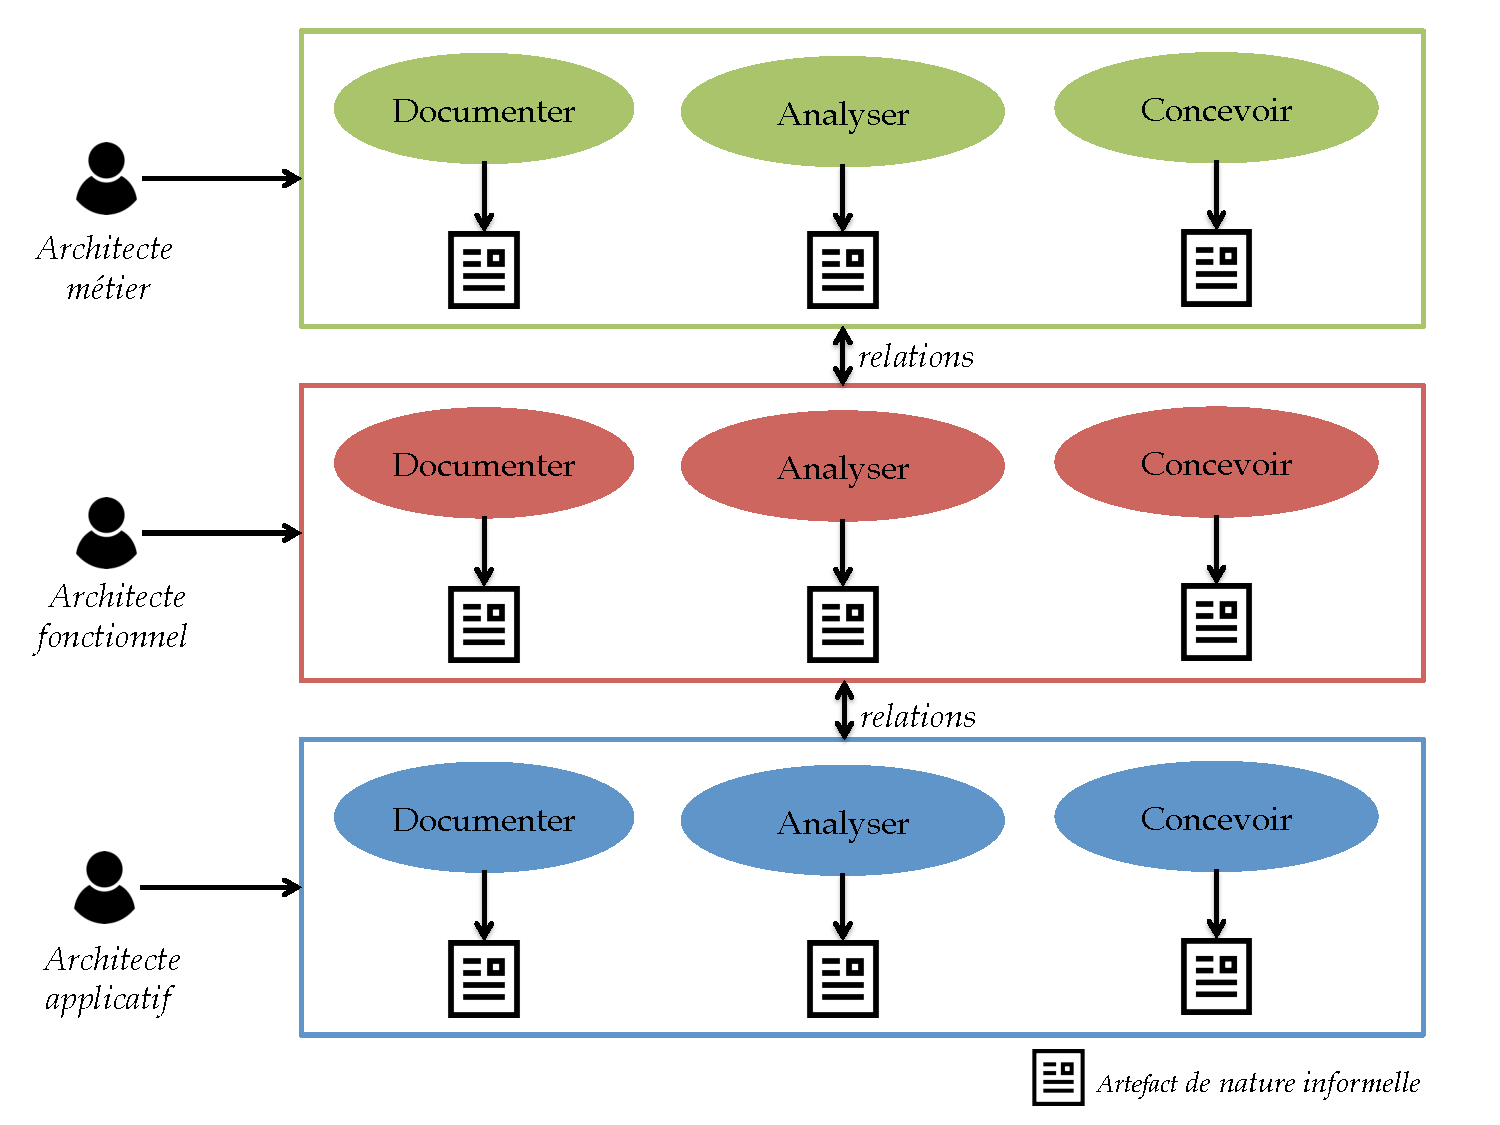
\includegraphics[width=1\textwidth]{figures/4_demarche/pratique_courante_ea.pdf}
     \end{center}
     \caption{Activités et artefacts produits pour les différentes vue d'une architecture d'entreprise}
     \label{fig:limites_ea}
\end{figure}

L'EA englobe ces différentes activités et les décline selon les différentes
vues d'architecture (voir chapitre~\ref{ch:EA}) comme l'illustre la
figure~\ref{fig:limites_ea}. Les artefacts produits par les différentes
activités des différentes vues sont donc d'autant plus nombreux. Ces artefacts
adressent les préoccupations de différentes parties-prenantes.

La revue de la littérature relative à l'EA, nous a permis de catégoriser ces
parties-prenantes en identifiant un rôle par vue d'architecture. Chacun de ces
rôles a pour mission de construire une vision holistique au regard de ses
propres préoccupations. C'est donc pour cette raison que nous identifions un
architecte par vue~:

\begin{description}
    \item[l'architecte métier]
    Le rôle de l'architecte métier consiste à documenter, analyser et concevoir
    des processus métier permettant à l'entreprise de réaliser sa stratégie.
    Il orchestre les processus métier et les flux d'information en cohérence
    avec la stratégie pour aboutir à l'architecture métier de l'entreprise~;

    \item[l'architecte fonctionnel]
    Le rôle de l'architecte fonctionnel consiste à documenter, analyse et
    concevoir les blocs fonctionnels qui réalisent les processus de
    le vue métier. Il orchestre ces blocs fonctionnels et les flux d'informations
    qui circulent entre ces blocs pour aboutir à l'architecture fonctionnelle
    de l'entreprise~;

    \item[l'architecture applicatif]
    Le rôle de l'architecte applicatif consiste à documenter, analyser
    et concevoir les applications permettant d'implémenter les blocs
    de la vue fonctionnelle. Il doit assurer une bonne orchestration de ces
    applications et des informations échangées pour aboutir à l'architecture
    applicative de l'entreprise.
\end{description}

Les architectes sont essentiellement tenus de documenter, d'analyser et de
concevoir des architectures selon leurs propres perspectives, en assurant les
critères de \emph{cohérence interne} à chacune des vues mais en respectant
aussi les critères de \emph{cohérence externe} avec les autres vues. Cependant,
la nature informelle des artefacts impliqués dans les différentes activités
d’architecture rend difficile le maintien de cette cohérence.

Comme exposé dans la problématique (chapitre~\ref{ch:problematique}), les
entreprises doivent constamment faire évoluer leurs stratégies. En conséquence,
l'architecture doit satisfaire, en plus des contraintes de cohérence, des
contraintes de souplesse et de réactivité. Mais souvent, la nature informelle
des artefacts d’architecture ne permet pas de satisfaire aux contraintes de
souplesse et de réactivité.

Dans le cadre d'une démarche IDM, ce type d'artefacts est qualifié de purement
contemplatif. L'IDM traite la question des modèles purement contemplatifs dans
le contexte particulier du génie logiciel, en proposant une approche
unificatrice par les modèles~\cite{jezequel2006genie}. Une revue comparative
des littératures relevant de l'IDM et des pratiques courantes de l'EA, nous
amène à envisager l'IDM comme cadre méthodologique et technologique pour l'EA.
Dans la partie suivante, nous faisons donc le parallèle entre les deux
disciplines afin de justifier le recours à une démarche IDM  pour traiter les
limites  des pratiques actuelles d'EA.

\subsection{L'Ingénierie Dirigée par les Modèles~:\\ un cadre méthodologique et technologique}

    La problématique que traite les présents travaux (voir
    chapitre~\ref{ch:problematique}) est résumée dans la question suivante~:

    %\begin{framed}
    {\bfseries Quels méthodes, modèles et outils adopter pour simuler une architecture d'entreprise afin de la valider?}
    %\end{framed}

    Pour répondre à cette problématique, nous avons adopté une démarche IDM.
    Nous commençons par démontrer la pertinence de ce choix de démarche
    au regard de la problématique traitée.  Nous décrivons ensuite la dite démarche.

            \subsubsection{De la cohérence entre démarche adoptée et
    problématique traitée}

    Le recours à une démarche IDM tire sa légitimité de la mise en
    évidence des caractéristiques communes des deux disciplines que
    sont le génie logiciel et l'EA. La démarche IDM est certes originellement développée
    pour le génie logiciel. Cependant, nous identifions un nombre de similarités
    entre les deux disciplines justifiant l'adéquation d'une démarche IDM pour l'EA.

    Premièrement, l'EA tout comme le génie logiciel, cherchent à construire
    des systèmes manipulant de l'information. Il s'agit d'un système à
    logiciel prépondérant pour le génie
    logiciel~\cite{jezequel2012ingenierie} et du système entreprise pour l'EA.
    Or les entreprises se mettent de plus en plus à produire et à
    consommer de l'information \cite{zachman1997enterprise}, à
    commencer par les Smart Grids dont le fonctionnent reposent sur la
    mise en réseau, au sens informatique, des équipements électriques. Certains auteurs
    évoquent même une nouvelle ère de l'information qui sonnerait
    la fin de l'ère d'industrialisation en inscrivant les entreprises dans une économie
    de l'information~\cite{toffler1981third}~\cite{webster2014theories}.

    Deuxièmement, l'EA et le génie logiciel comportent des activités
    similaires comme l'expression des besoins et des objectifs, l'analyse,
    la conception, la maintenance, la documentation, l'implémentation ou encore
    la validation. Ces activités reste similaires dans leur nature même
    si elles ne portent pas sur le même système, en l'occurrence l'entreprise et
    le logiciel.

    Troisièmement, en génie logiciel, les partie-prenantes sont
    confrontés aux limites de ces artefacts hétérogènes et de nature informelle (mise à
    part le code) produits au différentes étapes du cycle de vie du système (documentation,
    spécifications, etc.). Jézéquel et al. \cite{jezequel2006genie} affirment
    que «~ces artefacts donnent de multiples points de vue sur le
    logiciel en cours de développement et, en pratique, sont souvent
    indépendants les uns des autres~», et que le problème est «~d’être
    capable d'assurer une cohérence entre ces vues, ou au minimum une
    traçabilité entre les éléments des différents artefacts~».
    Comme exposé dans la partie précédente, le même problème se pose pour l'EA.

    %Quatrièmement, demande de ractivité et de soupelesse. Stratégie en évolution pour l'EA et spect pouvante pour le génie logiciel

    Similarité des domaines et communauté des objectifs légitiment
    donc pleinement le recours à l'IDM comme cadre
    méthodologique et technologique pour répondre à la problématique de
    cette thèse.

    \subsubsection{Contribution de l'Ingénierie Dirigée par les Modèles\\à l'Architetcure d'Entreprise}

    La vision que nous souhaitons transmettre dans cette partie est la suivante~:
    l'Ingénierie Dirigée par les Modèles est un moyen d'unifier les activités
    et les artefacts de l'Architecture d'Entreprise. Ainsi unifiée, l'EA parviendra à réaliser
    pleinement ses objectifs d'alignement effectif et d'accompagnement efficace de
    l'entreprise tout au long de sa trajectoire.

    L'IDM offre à cet effet un nombre de méthodes et de technologies permettant d’homogénéiser
    les vues d'architecture tout en gardant la possibilité d'utiliser la technologie ou la représentation
    la mieux adaptée à chaque vue.
    C'est par la méta-modélisation que l'IDM parvient à cette unification. Les métamodèles
    permettent de formaliser les langages de modélisation  et d'automatiser ainsi
    le traitement des modèles.
    Il est alors possible de vérifier automatiquement la conformité de ces modèles au métamodèle.
    Le métamodèle renferme les règles d'association des concepts manipulés par les modèles.
    La relation de conformité peut alors servir à assurer la cohérence globale de l'EA.
    Les modèles d'architecture manipulés deviennent alors productifs,
    par opposition aux modèles contemplatifs habituellement utilisés. Les modèles productifs sont
    en réalité des modèles exécutables qui peuvent être transformés en d'autres modèles exécutables
    selon les besoins de modélisation.

    Le recours intensif aux modèles exécutables dans les activités d'EA
    pour chacune des vues d'architecture permet de créer une architecture d'entreprise
    souple et réactive à l'évolution de la stratégie d'entreprise. Les modèles d'une vue être automatiquement
    raffinés en modèles cible pour la vue d'en dessous grâce aux transformations de modèles. Les modèles
    exécutables et les transformation de modèles permettront d'automatiser
    les activités d'EA telles que l'analyse de la structure et du comportement
    ainsi que la mise à jour.

    L'IDM permet toutes ces possibilités par la formalisation d'un métamodèle pour

    Nous détaillerons plus en détails les possibilités d'utilisation des méthodes et technique de l'IDM
    dans la suite de ce chapitre. Mais nous présentons d'abord la démarche IDM mise en
    œuvre pour la création du métamodèle EA2M.

    \subsubsection{Démarche mise en œuvre}

    S'il n'existe pas de démarche standardisée pour mettre en œuvre
    l'IDM \cite{barbier13phd}, les différents auteurs conviennent néanmoins de la
    nécessité  de commencer par analyser le domaine d'application~\cite{jezequel2012ingenierie}.
    Dans notre contexte, il s'agit de la découverte des pratiques
    d'EA dans le contexte des Smart Grids. L’appréhension du domaine a
    pour objectif d'identifier les concepts essentiels en EA ainsi que leurs
    règles d'association afin de concevoir un métamodèle du domaine traité. La
    figure~\ref{fig:demarche_idem} est une représentation de la démarche IDM
    mise en œuvre pour mener les travaux de cette thèse.

    Il est important de préciser que la définition du métamodèle EA2M s'est faite de manière
    itérative~: commencer par quelques concepts en précisant leurs relations,
    créer des modèles conformes à ce métamodèle, tester le modèle obtenu par rapport
    aux attentes du domaine, enrichir à nouveau le métamodèle et ainsi de suite.

    L'IDM permet par transformation de modèle de générer de code des applications
    finales. Nous avons donc utilisé les transformations de modèle pour éprouver la pertinence du métamodèle
    EA2M sur un système informatique au fil des itérations.


    \begin{figure}[!ht]
         \begin{center}
        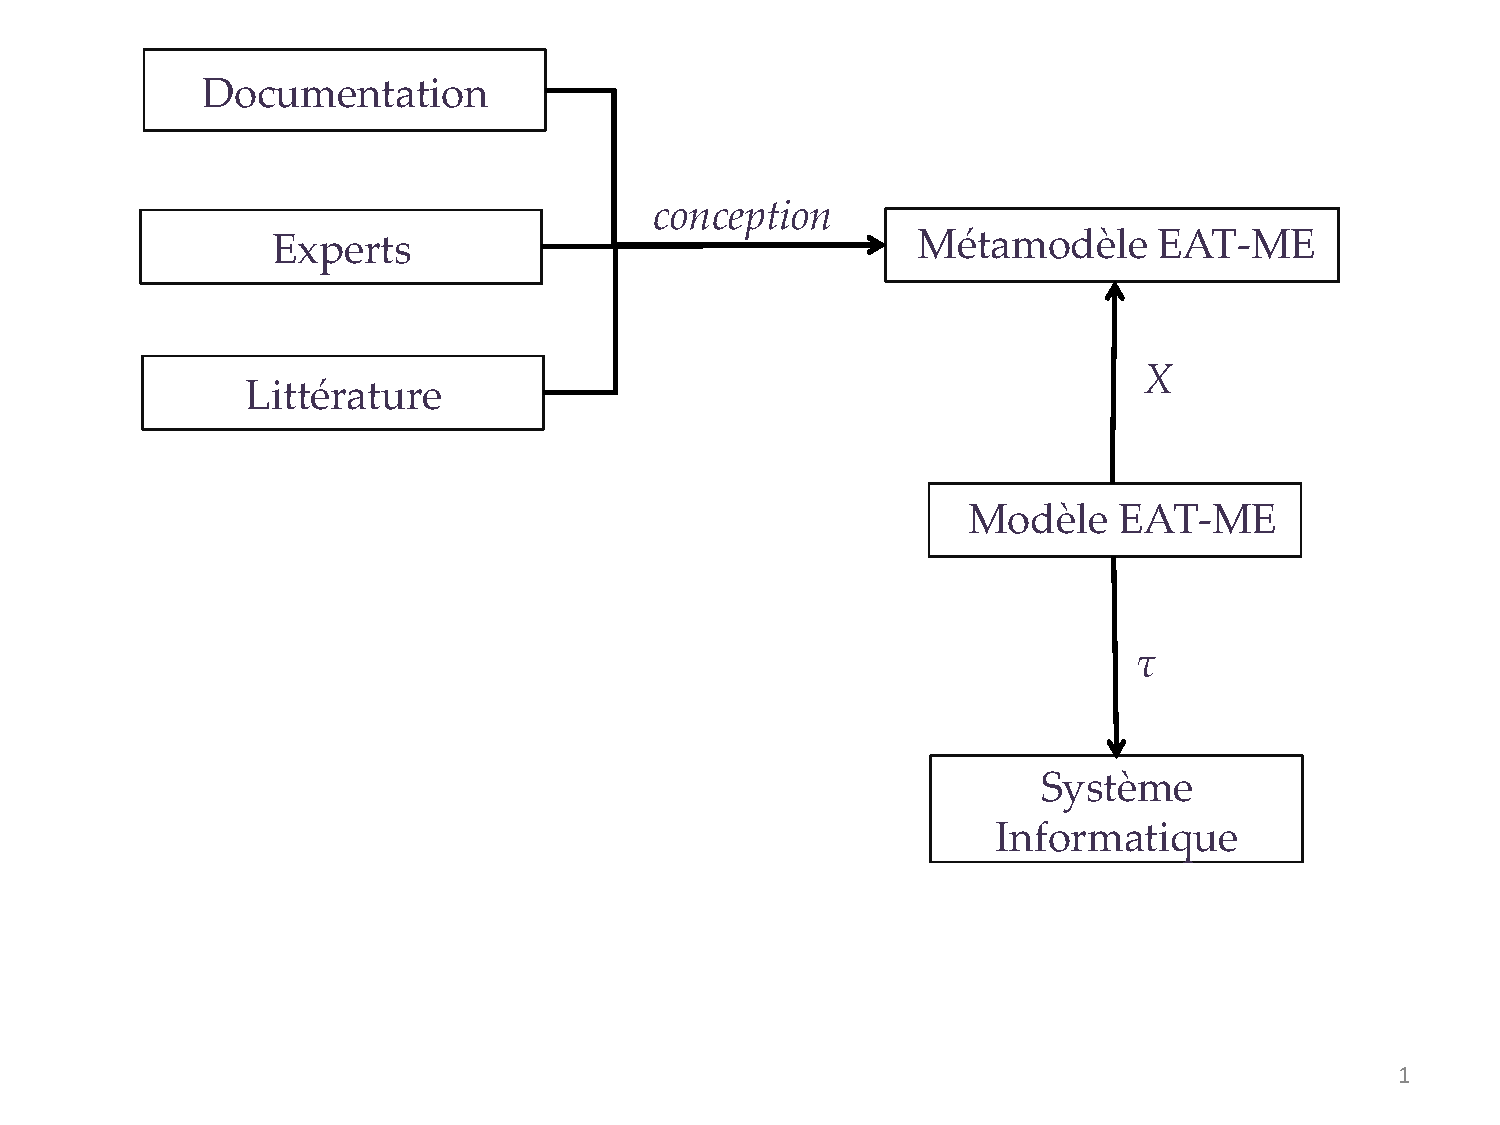
\includegraphics[trim=0cm 4cm 0cm 0cm, width=0.8\textwidth]{figures/4_demarche/demarche_idm.pdf}
         \end{center}
         \caption{Mise en œuvre d'une démarche IDM pour l'Architecture
         d'Entreprise}
         \label{fig:demarche_idem}
    \end{figure}

    L'appréhension du domaine de l'EA a été menée de différentes manières~:

    \begin{itemize}

        \item par l'analyse des documentations d'architecture utilisées dans divers projets Smart
    Grids. Nous avons tenu à examiner les pratiques d'EA dans le contexte des Smart Grids
    pour mieux mettre en œuvre notre approche par la suite~;

        \item par les entretiens menés avec les experts d'EA du département MIRE (dont notamment
    plusieurs personnes certifiées \gls{togaf}) ainsi que des chefs de projets Smart Grid,
    des membres de groupes de normalisation Smart Grid de la \gls{cei}\footnote{http://www.iec.ch}~;

        \item par une revue de la littérature portant sur l'EA de manière générale,
        écrite par des chercheurs et des praticiens.

    \end{itemize}

La revue de la littérature a été présentée dans le chapitre~\ref{ch:EA}.
Dans la suite de ce chapitre, nous présentons donc l'analyse du domaine à travers l'étude
de la documentation à laquelle nous avons eu accès et les entretiens menées avec les différents
experts et praticiens du domaine.


\section{Analyse du Domaine}
%La découverte des Smart Grids a été menée de plusieurs manières. Hypothèse forte
% Le parallèle entre une entreprise et un projet Smart Grid cycle de vie les
%spec co = EA forte mais légitime

%Avant d'aboutir à, Hypothèse : L'entreprise comme un projet - Fractal Entreprise
%= petit projet Structure fractale
    \subsection{L'Architecture d'Entreprise pour les Smart Grids}
    \subsubsection{Démonstrateurs européens}
    \label{sec:DemonstrateursSG}

Tout d'abord, nous avons étudié les spécifications des démonstrateurs Smart Grid
européens et en particulier celles de ADDRESS et PREMIO. Le choix de ces deux
démonstrateurs est expliqué par la participation du département MIRE à ces deux
projets, ce qui a facilité l'accès aux documents officiels.

%\footnote{http://www.smartgrids-
%\cre.fr/media/documents/dossiers/zonesinsulaires/ProjetR\&DAddress.pdf}
%\footnote{http://www.smartgrids-
%\cre.fr/media/documents/evenements/130618$_$Presentation$_$Prufer.pdf}


Le projet ADDRESS regroupe 25 partenaires dans 11 pays. L'objectif visé est
d'améliorer l'efficacité, la sécurité et la qualité de leur alimentation en
électricité dans un contexte de forte croissante de la participation des
énergies renouvelables à la production d'électricité. Pour cela, des
technologies sont développées pour gérer la consommation d'électricité des
clients résidentiels et professionnels.

Le projet PREMIO vise à optimiser la gestion globale du réseau électrique de la
région Provence-Alpes-Côte d'Azur (PACA) en intégrant les TIC et en
expérimentant~:
\begin{itemize}
	\item la production locale de l'énergie~;
	\item l'effacement~: il s'agit de baisser ou couper la consommation des utilisateurs
    sans en dégrader le confort~;
	\item stockage/déstockage de la chaleur ou du froid.
\end{itemize}

L'étude de la documentations des deux projets a été utile à la compréhension des
enjeux Smart Grids et à l'exploration des pratiques de spécification de ce type
de grand projet impliquant plusieurs partenaires. Les deux spécifications se
présentent sous la forme de contenu textuel agrémenté de diagrammes de cas
d'utilisation et de diagrammes de séquences UML. La spécification reste
cependant essentiellement textuelle avec quelques dessins d'architecture, donnant
lieu à une représentation purement contemplative. En outre, aucun lien de
traçabilité entre l'architecture proposée dans la spécification et son
implémentation réelle n'est explicité.

\subsubsection{Normalisation de \textit{Use Case} Smart Grids}
\label{sec:ENEL}

La normalisation de \textit{Use Case} ou de cas d'utilisation consiste à
imposer un canevas pour la spécification des cas d'utilisation Smart Grid puis à
faire le mapping entre cette spécification et le cadre d'architecture
\gls{sgam}. Le \gls{sgam}, spécialisé dans l'architecture des Smart Grids, est
présenté dans le chapitre~\ref{ch:EA}.

La normalisation de \textit{Use Case} est utilisée par le projet européen
GRID4EU\footnote{http://www.grid4eu.eu/} qui rassemble six démonstrateurs Smart
Grid différents. Les \textit{use case} ainsi normalisés, sont ensuite mis en
correspondance avec le cadre d'architecture \gls{sgam}. La normalisation des use
case dans le cadre de GRID4EU, a été faite après l'implémentation des six
démonstrateurs pour comparer les retours d'expérience. Nous retenons, en
particulier, le démonstrateur de la société nationale d'électricité italienne
(\gls{enel}) et son use case portant sur la régulation de tension des réseaux de
distribution présentant une forte pénétration de \gls{der}. C'est le cas d'application
de la norme et du cadre \gls{sgam} le plus fourni et abouti du projet GRID4EU.
L'analyse des documents de normalisation et des spécifications de projets
européens appliquant ces normes est à l'origine de plusieurs constatations.

D'une part, dans le \gls{sgam} la traçabilité entre les vues n'est pas directe.
Elle est au contraire assurée par la superposition des différentes vues
d'architecture sur le \textit{Smart Grid Plan}. Ce dernier décrit un réseau
électrique selon deux composantes~: physique et organisationnelle. La
figure~\ref{fig:enel_sgplan} illustre une projection de la vue fonctionnelle et
de la vue technique (appelée vue composant dans le \gls{sgam}), telles que
définies par le démonstrateur d'\gls{enel} pour GRID4EU, sur le \textit{Smart
Grid Plan}. Pour tirer les liens de traçabilité entre deux vues, il faut donc
les superposer en même temps sur le \textit{Smart Grid Plan}. La normalisation
de \textit{Use Case} Smart Grid préconise l'utilisation du langage UML mais une
grande partie des \textit{Use Cases} est spécifiée sous la forme de texte
accompagné de quelques diagrammes d'activité ou de séquence.

\begin{figure}[!ht]
    \begin{center}
     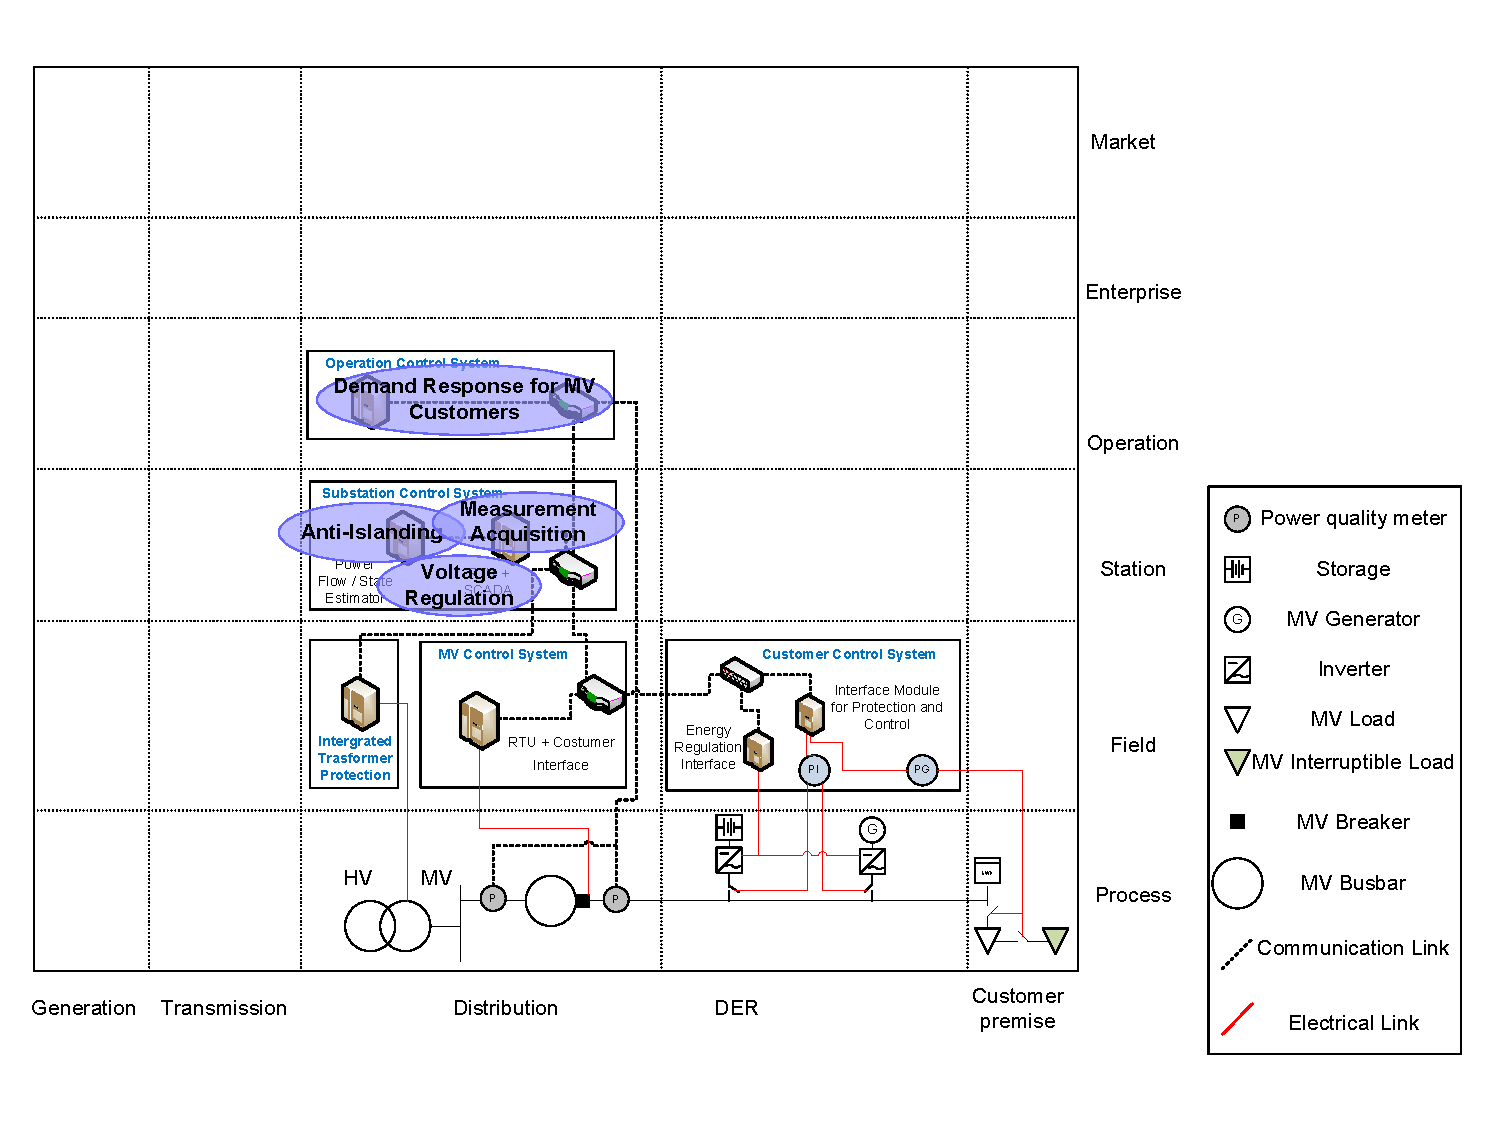
\includegraphics[trim=0cm 1cm 0cm 1cm, width=1\textwidth]{figures/4_demarche/enel.pdf}
    \end{center}
    \caption{Projection de la vue fonctionnelle du démonstrateur \gls{enel} de
GRID4EU sur le \textit{Smart Grid Plan}} \label{fig:enel_sgplan}
\end{figure}

D'autre part, il existe un grand déséquilibre entre (1) la spécification des
différents démonstrateurs (2) le soin apporté à la description d'une vue au sein
d'un même démonstrateur. En effet, certaines équipes détaillent leur cas
d'utilisation plus que d'autres.
%les équipes n'aime pas les nouvelles méthode}s / cadres de travail ref frameworks.
De plus, cet exercice ayant été mené par des équipes dont le profil est
fortement technique, les vues composant et communication du SGAM sont souvent
plus fournies que la vue métier par exemple.

Bien que le démonstrateur d'\gls{enel} soit le plus en avance en terme de
normalisation de \textit{Use Case}, l'analyse des spécifications de la
régulation de tension sur un réseau électrique n'a pas été suffisante à
l'appréhension de cette problématique sans connaissances préalable sur le
fonctionnement des réseaux de distribution. Pour cette raison, et afin de
collecter plus d'informations sur le sujet, les spécifications des projets
auxquels a participé le département \gls{mire} et qui abordent la régulation de
tension, ont été analysés.


\subsubsection{Projets de recherches et développement}

Le contexte de cette thèse CIFRE a favorisé les échanges avec les experts et les
ingénieurs-chercheurs de EDF R\&D en général, et du département \gls{mire} en
particulier. Nous avons ainsi eu accès aux documents de spécification relatifs à
un projet de régulation de tension de réseau de distribution. Ces documents sont
pour l'essentiel textuels. Des schémas de réseaux électriques et des courbes de
charges viennent illustrer les grands principes de la régulation de tension
mise en place. Le projet R\&D a abouti à l'implémentation d'une maquette de
simulation développée sous
Simulink\footnote{http://fr.mathworks.com/products/simulink/}. Les algorithmes
de régulation sont écrits en C++.

Outre la compréhension des principes de la régulation de tension, l'étude de
terrain a pour objectif de mener une étude sociologique des pratiques
d'architecture au niveau des projets Smart Grids. Quelques entretiens ont été
menés avec le développeur C++ et des experts de la régulation de tension. Les
experts techniques interrogés utilisent leurs propres langages de modélisation
(automates programmables) et d'implémentation (C++). Ils sont de plus peu
sensibles aux problématiques soulevées par l'EA. En effet, ils n'avaient pas
connaissance du \gls{sgam} ni de la normalisation de \textit{Use Case} pour la
régulation de tension des réseaux de distribution.
%Ceci peut être expliqué en partie par le fait qu'ils traitent des
%problématiques électrotechniques pointues.

Partant de ce constat et de l'émergence des problématiques liées au véhicule
électrique, notre étude terrain se porte alors sur le projet de la gestion
d'une flotte de véhicules électriques. Ce projet est en effet transverse touche plusieurs processus métier de
l'entreprise. D'une part, la flotte de véhicules est indispensable à la tournée
des agents EDF. D'autre part, leurs recharges impliquent un changement de
paradigme sans précédent dans le fonctionnement des réseaux électriques, comme
expliqué dans le chapitre \ref{ch:problematique}.

Cependant, la recharge des véhicules électriques relève encore une fois du
domaine purement électrotechnique. Le cas métier de la gestion d'une flotte de
véhicules électrique a l'avantage de toucher l'ensemble de l'entreprise~: du
gestionnaire de la flotte, à l'agent qui utilise le véhicules pour sa tournée,
en passant même par le responsable des tournées. De plus, même s'il s'agit d'un
projet de R\&D, celui-ci a abouti à une implémentation testée sur une petite
agence de La Poste, contrairement à au projet R\&D pour la régulation de
tension qui se limite à la simulation.

Les documents de spécification du projet de gestion d'une flotte de véhicules
sont pour l'essentiel textuels. Cependant, des \textit{slides} de présentation
détaillent (1)~les blocs fonctionnels principaux et leur décompositions en
fonctions (2)~les flux d'information entre ces blocs (3)~les équipes chargées
de les implémenter. Cette présentation illustre l'importance pour les équipes
de projet d'établir des liens clairs, d'une part entre les aspects «~donnée~»
et «~traitement~», et d'autre part entre la vue fonctionnelle et la vue
applicative.

Cependant, le support de présentation n'étant pas auto-portant, un entretien
avec la chef de projet et avec d'autres membres de l'équipe a été nécessaire
pour connaitre les objectifs métier du projet car ces derniers ne sont pas
explicités sur les supports de présentation. Il s'avère que l'objectif métier
était d'obtenir le meilleur retour sur investissement
(ROI\footnote{\textit{Return On Investment}}) possible de l'intégration de
véhicules électriques dans la flotte de l'entreprise.

Ces entretiens ont en outre permis d'identifier quelques problèmes rencontrés
sur le terrain que l'équipe de projet n'a pas pu anticiper. Par exemple, l'étude
préalable n'a pas tenu compte d'un facteur sociologique important. En effet,
les agents de La Poste ont l'habitude d'effectuer leur tournée quotidienne avec
une voiture thermique qui leur est attribuée sur l'année de manière à ce qu'ils
puissent garder leurs équipements de travail dans le véhicule. Or avec les
contraintes d'autonomie associées à l'usage de véhicules électriques,
l'affectation d'un véhicule à un agent dépend de la distance de sa tournée,
l'obligeant ainsi à constamment déplacer son matériel et détériorant ses
conditions de travail.

\subsection{Identification des concepts}
    \label{sec:conceptualisation}

    Un métamodèle est un modèle du langage de modélisation qui sert à décrire les modèles.
    Or l'activité de modélisation est guidée par l’intention du modélisateur.
    Par conséquent, il convient de définir clairement nos intentions de modélisation
    avant de caractériser les concepts retenus pour le métamodèle EA2M.

    D'abord, nous cherchons à caractériser les concepts essentiels et indispensable à la
    modélisation d'une vue d'architecture en mettant en évidence les caractéristiques communes
    aux artefacts utilisés par les praticiens. En effet, le métamodèle est un moyen d'unifier
    l'ensemble des artefacts employée dans les diverses activités d'EA.

    Ensuite, l’objectif de EA2M est de permettre de vérifier la cohérence internes à une vue mais
    aussi la cohérence entre deux vues d'architecture. Il est donc indispensable de représenter
    ces liens de cohérences dans le métamodèle. Nous expliquons dans la suite l'importance
    d'expliciter ces liens pour l'analyse de la structure et du comportement de l'architecture

    Enfin, nous cherchons à automatiser la manipulation des modèles d'architecture à travers
    la mise en œuvre de transformation de modèle. Il convient de de spécifier dans le modèle
    d'architecture l’existence ces transformations de ces transformations et leur utilité.)]

    Les approches par points de vue sont adaptées à la modélisation
    de systèmes complexes comme les architectures d'entreprise, nous adoptons une
    approche par points de vue. Celle-ci facilite la conception des modèles par les
    acteurs impliqués en séparant leurs préoccupations respectives. Elle permet
    également de présenter les modèles obtenus, ainsi que les résultats d'analyse 
    de manière plus compréhensible, car chaque point de vue
    n'utilise que les concepts métier propres à chaque acteur, selon sa perspective.
    Ceci nous amène à identifier les premier concept qui est celui de \textbf{vue}. 
    Dans la suite, nous identifions les concepts nécessaires à la modélisation de
    chacune des vues traitées dans ces travaux.



    \subsubsection{Concepts identifiés pour la vue métier}

    La vue métier reflète la perspective de l'architecte métier. Ce dernier
    décrit l’organisation de l'entreprise en terme de \textbf{processus métier}.
    La figure~\ref{fig:concepts_vue_metier} illustre les concepts retenus pour la vue
    métier en les représentant sous un format libre.

    Un processus est une séquence
    de \textbf{tâches} métier produisant un résultat qui
    participe à la réalisation d'un ou de plusieurs \textbf{objectifs métier} de l'entreprise.
    Ce résultat doit donc être mesurable au regard de l'objectif qu'il remplit afin de l'évaluer.
    De plus, les tâches métier produisent et utilisent des \textbf{concepts métier}.


    \begin{figure}[!ht]
     \begin{center}
     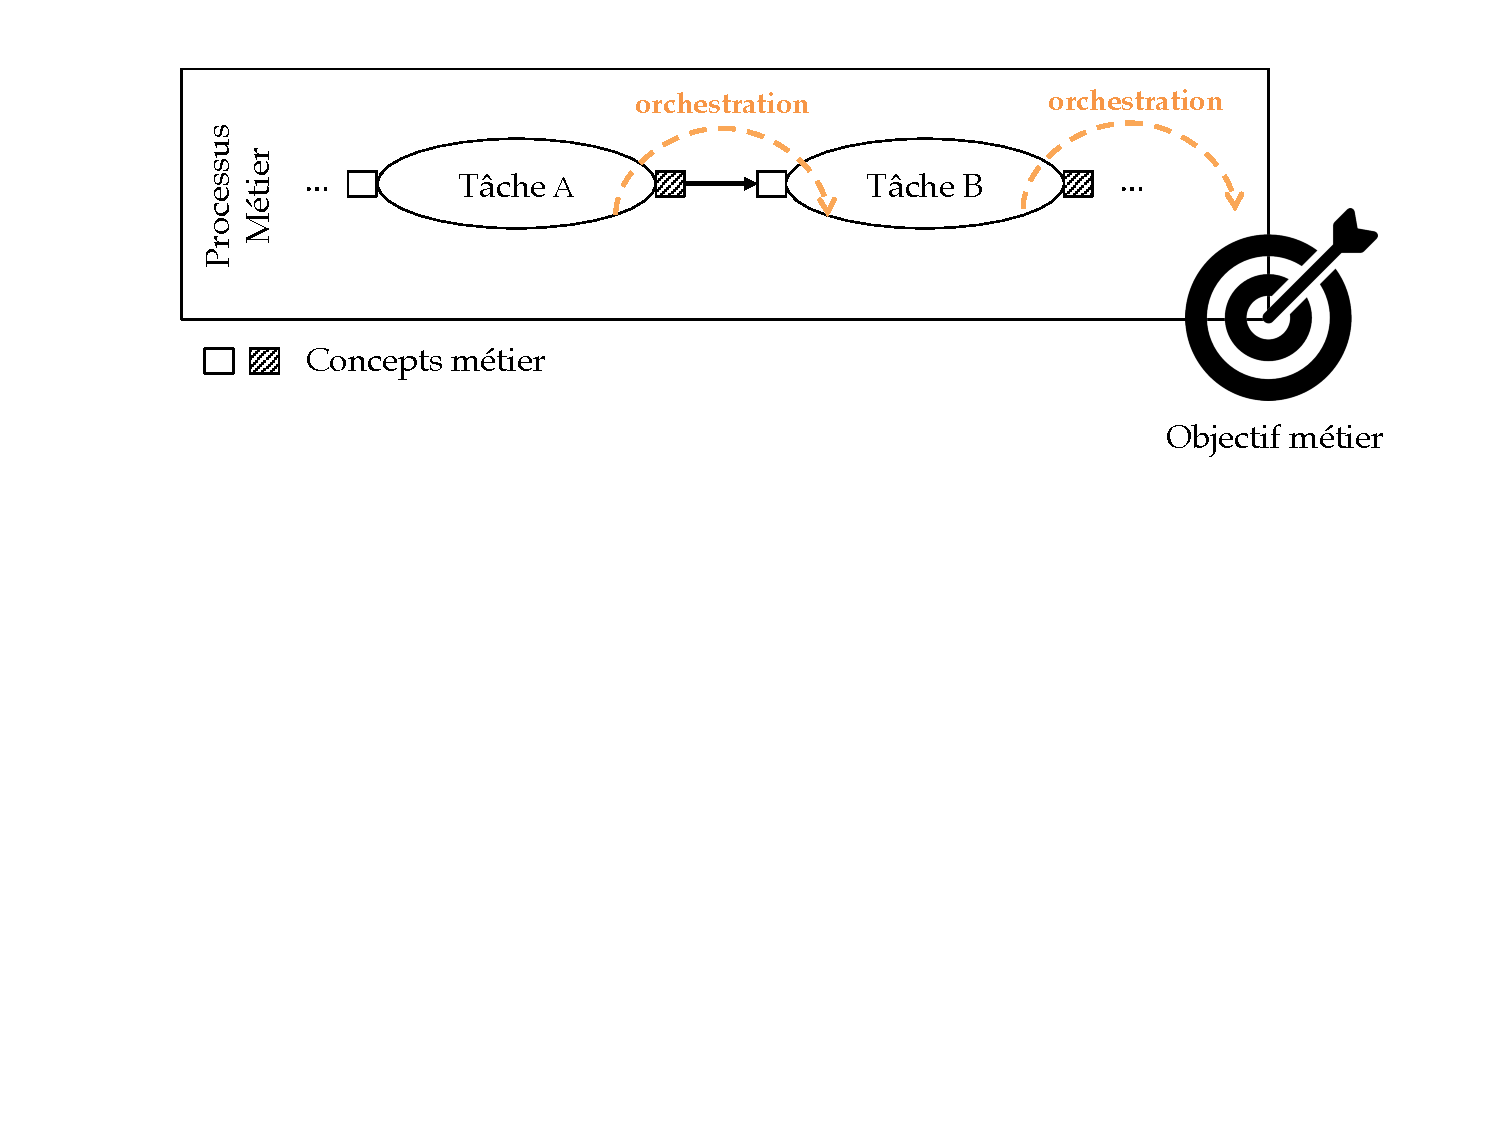
\includegraphics[trim= 0cm 11cm 0cm 0cm, width=1\textwidth]{figures/4_demarche/concepts_vue_metier.pdf} \end{center}
     \caption{Concepts identifiés pour le point de vue métier et représentés selon un formalisme libre}
     \label{fig:concepts_vue_metier}
    \end{figure}

    L'architecte métier doit organiser les différentes tâches métier en
    termes de processus cohérents et créateurs de valeur pour l'entreprise. À ce titre, les objectifs de chaque processus
    métier doivent être clairement identifiés et lui être associés.
    Si deux processus sont identifiés comme remplissant les mêmes processus métier, l'architecte métier
    peut alors les détecter grâce à ces relations et garantir ainsi la \textbf{cohérence interne }à la vue.

    Il doit en outre veiller à la bonne orchestration des processus métier
    mais aussi des tâches composant un processus pour garantir une bonne exécution des processus métier.
    L'orchestration des tâches et des processus est en grande partie garantie par le partage
    et la diffusion de l'information, c'est-à-dire des concepts métier, au sein de l'entreprise participant ainsi la cohérence
    interne de la vue métier.

    Dans le cas des très grandes entreprise, il est possible qu'un même concept métier
    soit référencé par deux noms différents par exemple, à la suite d'une fusion ou d'une acquisition par exemple.
    Le rôle de l'architecte métier est d'identifier cette incohérence, de mettre en œuvre les solutions requises pour
    la corriger et de la communiquer au reste de l'entreprise.
    Le concept métier est donc une entité de première importance pour la vue métier.

    \subsubsection{Concepts identifiés pour la vue fonctionnelle}

    La vue fonctionnelle est la pierre angulaire d'une architecture d'entreprise. C'est par elle que se fait la transition entre la vue métier très abstraite, et la vue applicative qui représente le système informatique.
    Elle joue de ce fait un rôle de premier plan dans la problématique d'alignement métier/IT mais surtout en tant
    qu'interface et interprète entre le métier et l'IT.

    La vue fonctionnelle reflète la perspective de l'architecte fonctionnel. Ce dernier doit spécifier les \textbf{fonctions}
    qui raffinent les tâches métier en les organisant en \textbf{processus fonctionnels}. Les tâches et les fonctions
    sont liés par des relations de \textbf{raffinement}.
    Les fonctions participent à atteindre des \textbf{objectifs fonctionnels}, qui eux mêmes raffinent les objectifs
    de la vue métier. Comme pour la vue métier, définir des relations explicites entre les processus fonctionnels
    et les objectifs qu'ils remplissent permet de vérifier qu'il n'y a pas de redondance ou de recouvrement
    et d'optimiser ainsi l'ensemble de l'architecture.

    \begin{figure}[!ht]
     \begin{center}
     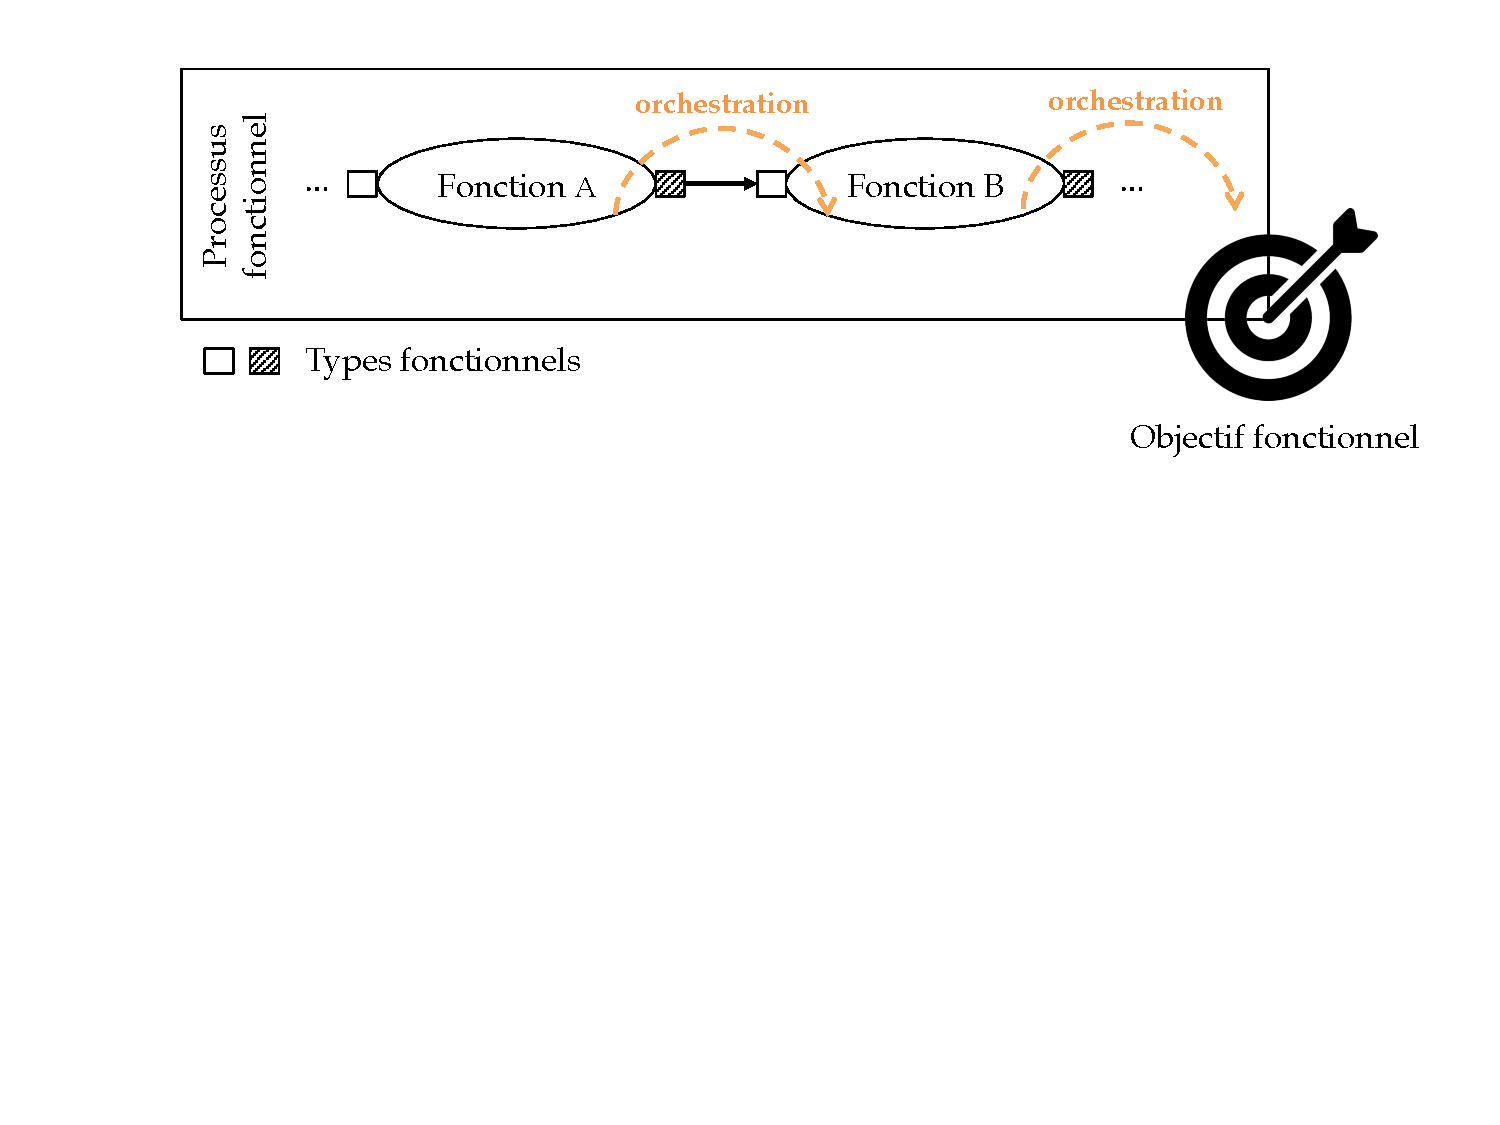
\includegraphics[trim= 0cm 11cm 0cm 0cm, width=1\textwidth]{figures/4_demarche/concepts_vue_fonctionnelle.pdf} \end{center}
     \caption{Concepts identifiés pour le point de vue fonctionnel et représentés selon un formalisme libre}
     \label{fig:concepts_vue_fonctionnelle}
    \end{figure}

    Les fonctions utilisent et produisent des \textbf{types fonctionnels}. L'orchestration d'un processus fonctionnel
    nécessite que le type fonctionnel en sortie d'une fonction soit compatible avec le type de donnée
    en entrée de la fonction suivante. La vue fonctionnelle doit donc permettre de vérifier cette compatibilité
    pour garantir une \textbf{cohérence interne}.
    Si un type $ T_{A} $ en sortie d'une fonction $ F_{A} $  n'est pas compatible avec le type en entrée
    $ T_{B} $ d'une fonction $ F_{B} $, l'architecte doit pouvoir détecter cette incompatibilité de type.
    Une transformation de modèle $t_{T_{A} \rightarrow T_{A}}$ peut alors être envisagée.

    Le types fonctionnels raffinent les concepts métier en donnant leur type, c'est-à-dire leurs différents attributs.
    Ce raffinement permet de vérifier que l'ensemble des concepts métier sont bien représentés dans la vue
    fonctionnelle et de vérifier ainsi que les informations de la vue fonctionnelle sont bien alignées avec
    celles de la vue métier et garantir ainsi une \textbf{cohérence externe} avec la vue métier.

    \subsubsection{Concepts identifiés pour la vue applicative}
    La vue applicative reflète la perspective de l'architecte applicatif. Ce derniers spécifie les \textbf{modules
    applicatifs} qui implémentent les fonctions de la vue fonctionnelle.
    L'objectif de cette vue est de garantir une \textbf{cohérence externe} entre la vue applicative et la vue fonctionnelle,
    en traçant les liens de \textbf{raffinement} entre fonctions et module. Cette
    traçabilité est garantie entre la vue métier et la vue applicative par transitivité et participe ainsi
    à maintenir l'alignement métier/IT.

    \begin{figure}[!ht]
     \begin{center}
     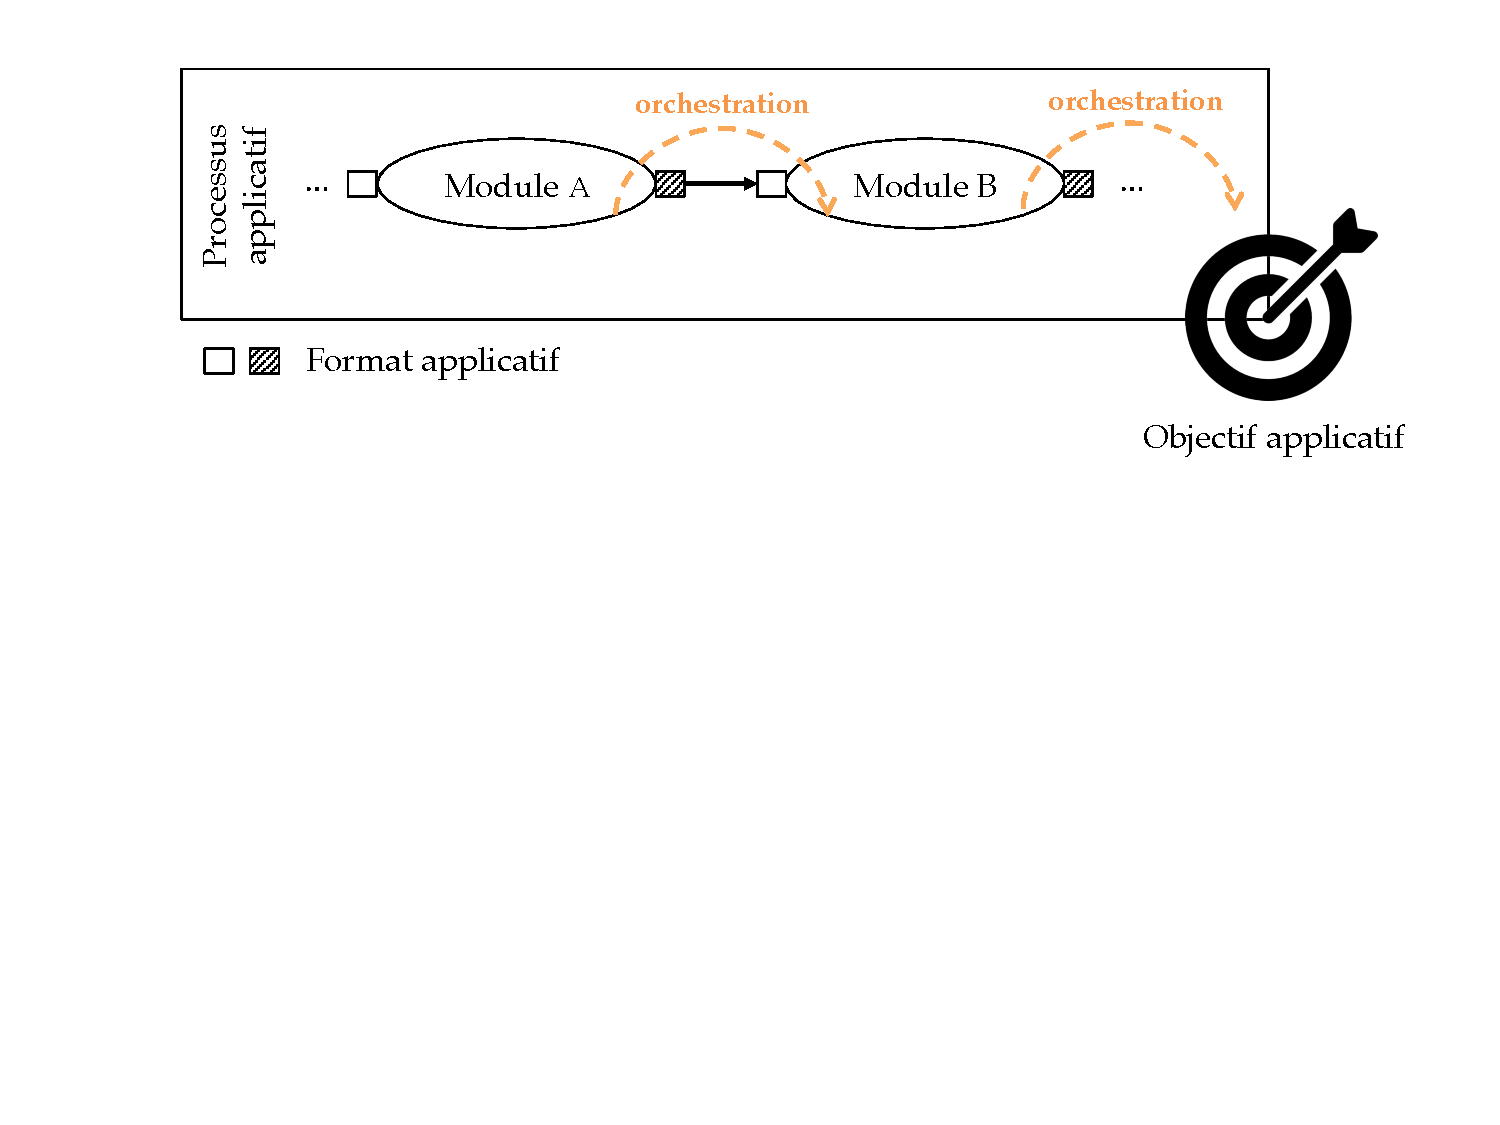
\includegraphics[trim= 0cm 11cm 0cm 0cm, width=1\textwidth]{figures/4_demarche/concepts_vue_applicative.pdf}
     \end{center}
     \caption{Concepts identifiés pour le point de vue applicative et représentés selon un formalisme libre}
     \label{fig:concepts_vue_applicative}
    \end{figure}

    Comme l'illustre la figue~\ref{fig:concepts_vue_applicative}, la vue applicative spécifie
    en outre les \textbf{formats applicatifs} manipulés par les modules. Expliciter
    ainsi les formats applicatifs permet de garantir une bonne orchestration des processus applicatifs. Par
    exemple, un module $M_{A}$ produit un format $F_{A}$ et
    un module $M_{B}$ prend en entrée un format $F_{B}$. Si les deux formats
    ne sont pas compatibles alors l'orchestration des deux modules n'est pas possible.
    Dans ce cas, l'architecte applicatif peut le détecter et mettre en place une \textbf{transformation de
    modèles} $t_{F_{A} \rightarrow F_{A}}$ pour traiter cette incompatibilité de format sans pour
    autant changer ses modules.

    La vue applicative permet de représenter l'architecture applicative d'une entreprise qui peut englober
    des centaines voire des milliers de modules et d'application. Formaliser ainsi cette vue permet de mener
    des analyses d'impact et de changement. Par exemple, les liens de traçabilité entre la vue métier et la
    vue applicative (via la vue fonctionnelle) permettent d'identifier les processus métier susceptibles d'être
    impactés par un changement de module applicatif. À l'inverse, il est possible d'identifier les modules
    applicatif impactés par un changement de processus métier.

    L'architecte fonctionnel doit spécifier les \textbf{objectifs applicatifs} que doit remplir chaque module. De
    cette manière il est possible de détecter les éventuelles applications redondantes ou celles qui
    ne participent plus à atteindre les objectifs de l'entreprise. Les objectifs applicatifs sont de plus dérivés
    des objectifs fonctionnels, eux mêmes dérivés des objectifs métier. Ainsi, il est possible de tracer
    explicitement la déclinaison des objectifs de l'entreprise sur l'ensemble de l'architecture pour contrôler
    la mise en œuvre d'une stratégie d'entreprise.

    L'analyse des pratiques de l'EA a permis d'identifier ces éléments indispensables à la mise en œuvre
    de méthode permettant de garantir la cohérence globale de l'architecture d'entreprise. Il est important
    de noter que nous avons repris l'approche ensembliste de Favre~\cite{favre2005foundations} en procédant
    par identification des caractéristiques communes des artefacts habituellement manipulés par
    les architectes d'entreprise contrairement à une approche ontologique qui vise à dresser un inventaire des
    connaissance du domaine.

    Cette démarche est d'autant plus justifiée que notre objectif premier n'est pas de modéliser une architecture
    d'entreprise dans ces moindres détails mais de prendre en comptes les éléments indispensables à
    la vérification de la cohérence de l'ensemble de l'architecture.

    Les concepts identifiés, directement issus l'analyse du domaine de l'EA, ont servi à la conception du
    métamodèle EA2M pour \emph{Enterprise Architecture MetaModel}.

\section{Le métamodèle EA2M}
    La conception du métamodèle EA3M a été menée de manière itérative. En partant de quelques concepts
    et en enrichissant le métamodèle à chaque itération. Des versions successives de ce métamodèle
    ont fait l'objet de publications (\cite{seghiri2015simulation} et \cite{seghiri2016executable}).
    L'analyse du domaine a été menée dans le cadre des projets Smart Grid, tout en confrontant systématiquement
    les concepts identifiés aux pratiques d'EA issues de la littérature. Le métamodèle EA3M a été conçu en gardant
    à l'esprit la possibilité de l'utiliser dans différents contextes et pas seulement pour les Smart Grids.

    \subsection{Éléments de base et cohérence \emph{intra-vue}}
    \label{sec:intravue}

    L'identification des concepts met en évidence les éléments de base nécessaires à la modélisation d'une
    architecture d'entreprise~: «~Information~», «~Action~» et «~Objectif~». Ces trois entités élémentaires permettent de décrire
    le contenu de chacune des vues d’architecture (métier, fonctionnelle et applicative).
    La figure~\ref{fig:core_concepts} illustre, sous la forme d'un diagramme de 
    classes, la partie\footnote{Nous fournissons des sous-parties du métamodèle pour des raisons de
    lisibilité} du métamodèle EA2M dédiée à la représentation de ces éléments.

    \begin{figure}[!ht]
    \begin{center}
    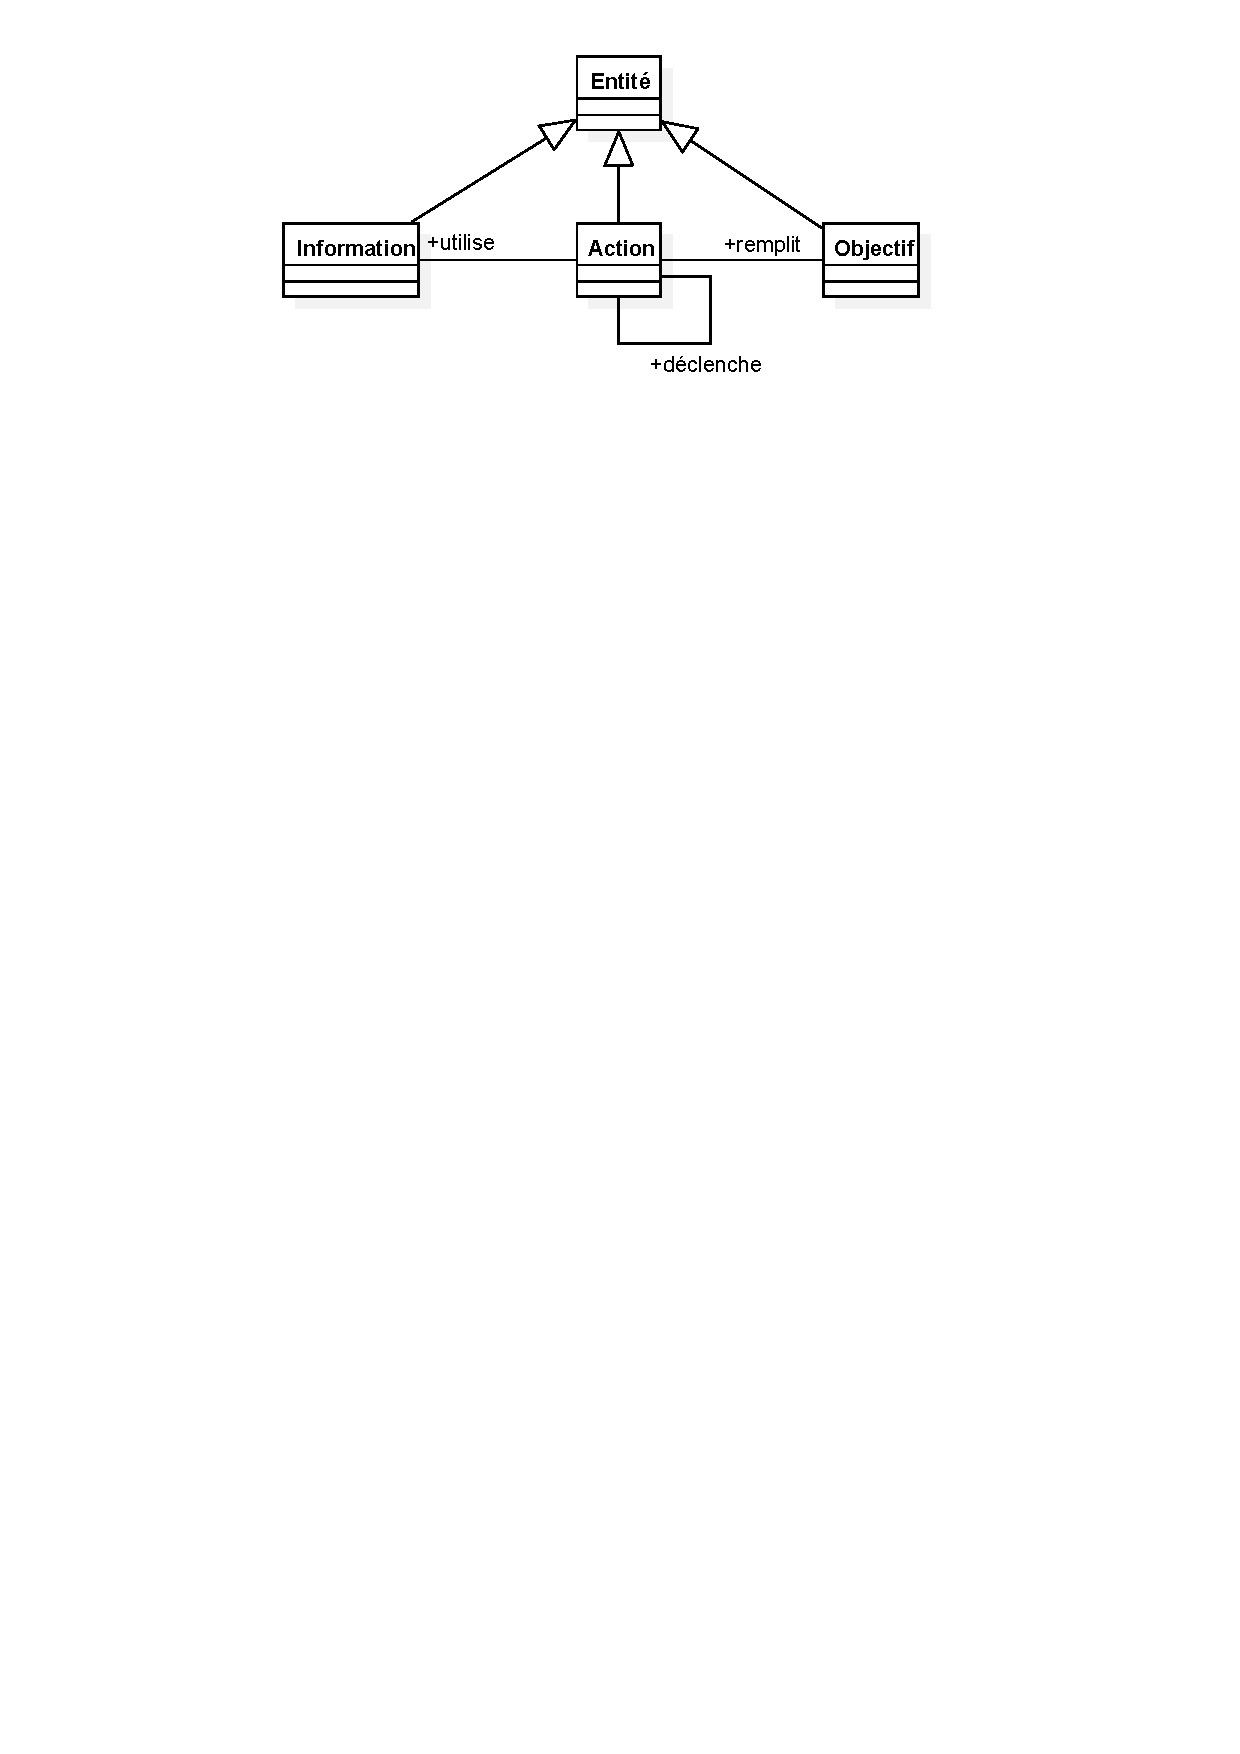
\includegraphics[trim= 0cm 23cm 0cm 0cm, width=1\textwidth]{figures/4_demarche/core_concepts.pdf}
    \end{center}
    \caption{Partie du métamodèle concernant les éléments de base et leurs relations} 
    \label{fig:core_concepts}
    \end{figure}

    EA2M n'a pas pour objectif la modélisation extensive des artefacts d'architecture mais se focalise sur
    l'abstraction des artefacts d'architecture à leur plus petit dénominateur commun pour pouvoir raisonner non plus
    sur la sémantique des éléments mais sur leur cohérence en termes de relations d'interdépendance. Par exemple, l'architecte métier 
    peut décrire des procédures composées de processus, eux-mêmes composés d'activités Le concept d'action peut aussi bien
    être utilisé pour décrire des procédures, des processus, des activités du moment qu'il s'agisse d'un élément d'architecture muni
    de comportement. Il suffit de se placer à la bonne échelle mais le concept d'action reste valable. Certains auteurs
    qualifient les systèmes obéissant à ce principe de systèmes à structure fractale~\cite{arsanjani2004service}.

    L'intérêt du métamodèle est de décrire la structure d'une architecture tout en maintenant une cohérence interne
    à chaque vue. Comme expliqué dans la section précédente, cette cohérence passe par la modélisation explicite
    de chaque entité afin de créer des liens de traçabilité indépendamment de l’exécution des processus.
    Par exemple, le fait de modéliser toutes les informations indépendamment des actions et de créer ensuite 
    des liens de traçabilité entre chaque action et les informations qu'elles utilisent permet de vérifier la compatibilité
    entre l'action et les informations impliquées, avant même d'exécuter le processus. Ainsi, si une action déclenche une autre
    action, il faut que l'information à la sortie de la première action soit compatible avec l'entrée de l'action déclenchée.
    En ce sens, les liens de traçabilité «~déclenche~» et «~utilise~»  garantissent
    une bonne orchestration des processus.

    La relation «~remplit~» permet de relier chaque action à ses objectifs et donne ainsi la possibilité 
    de suivre efficacement l’évolution
    de l'architecture au regard des objectifs définis. L'exploitation des liens de traçabilité entre actions et objectifs
    permet de (1) détecter les actions redondantes en termes d'objectif (2) déterminer les actions (et par transitivité 
    les informations) impactées par un changement d'objectif (3) et inversement, identifier les objectifs atteint
    par une évolution d'une action ou l'altération d'une information.

    La figure~\ref{fig:core_concepts_vue} illustre la partie du métamodèle consacrée 
    à la déclinaison des éléments de base (Action, Information, Objectif) en concepts spécialisés
    pour chacune des vues d'architecture (métier, fonctionnelle et applicative).
    Ces concepts ont d'abord été identifiés lors de l'analyse du domaine (voir section~\ref{sec:conceptualisation}), ainsi~:
    \begin{itemize}
    \item \q{Concept}, \q{Type} et \q{Format} héritent de \q{Information}~;
    \item \q{Tâche}, \q{Fonction} et \q{Module} héritent de \q{Action}~;
    \item \q{Objectif\_Métier}, \q{Objectif\_Fonctionnel} et \q{Objectif\_Applicatif} héritent de \q{Objectif}.
    \end{itemize}

    D'une part, les éléments de base du métamodèle nous ont amené à identifier la notion
    d'\textbf{aspect} d'une vue. Un aspect d'une vue est un sous-ensemble d'une vue dédié à la modélisation d'informations, d'actions
    ou encore d'objectifs.
    D'autre part, l'identification de relations entre les éléments de base nous a conduit à introduire une nouvelle vue~:
    la vue \textbf{intégration}. La vue intégration est dédiée à la modélisation des liens de traçabilité entre les éléments de base
    –~information, action et objectif~— à l'intérieur d'une même vue. 

    En ce sens, la vue intégration explicite les liens de \textbf{cohérence intra-vue},
    autrement dit, les liens de cohérence entre les aspects d'une même vue.
    Les notions de vue et d'aspect relèvent de la structure globale d'une architecture d'entreprise que
    nous détaillons dans la partie suivante.

    \begin{figure}[!ht]
        \begin{center}
    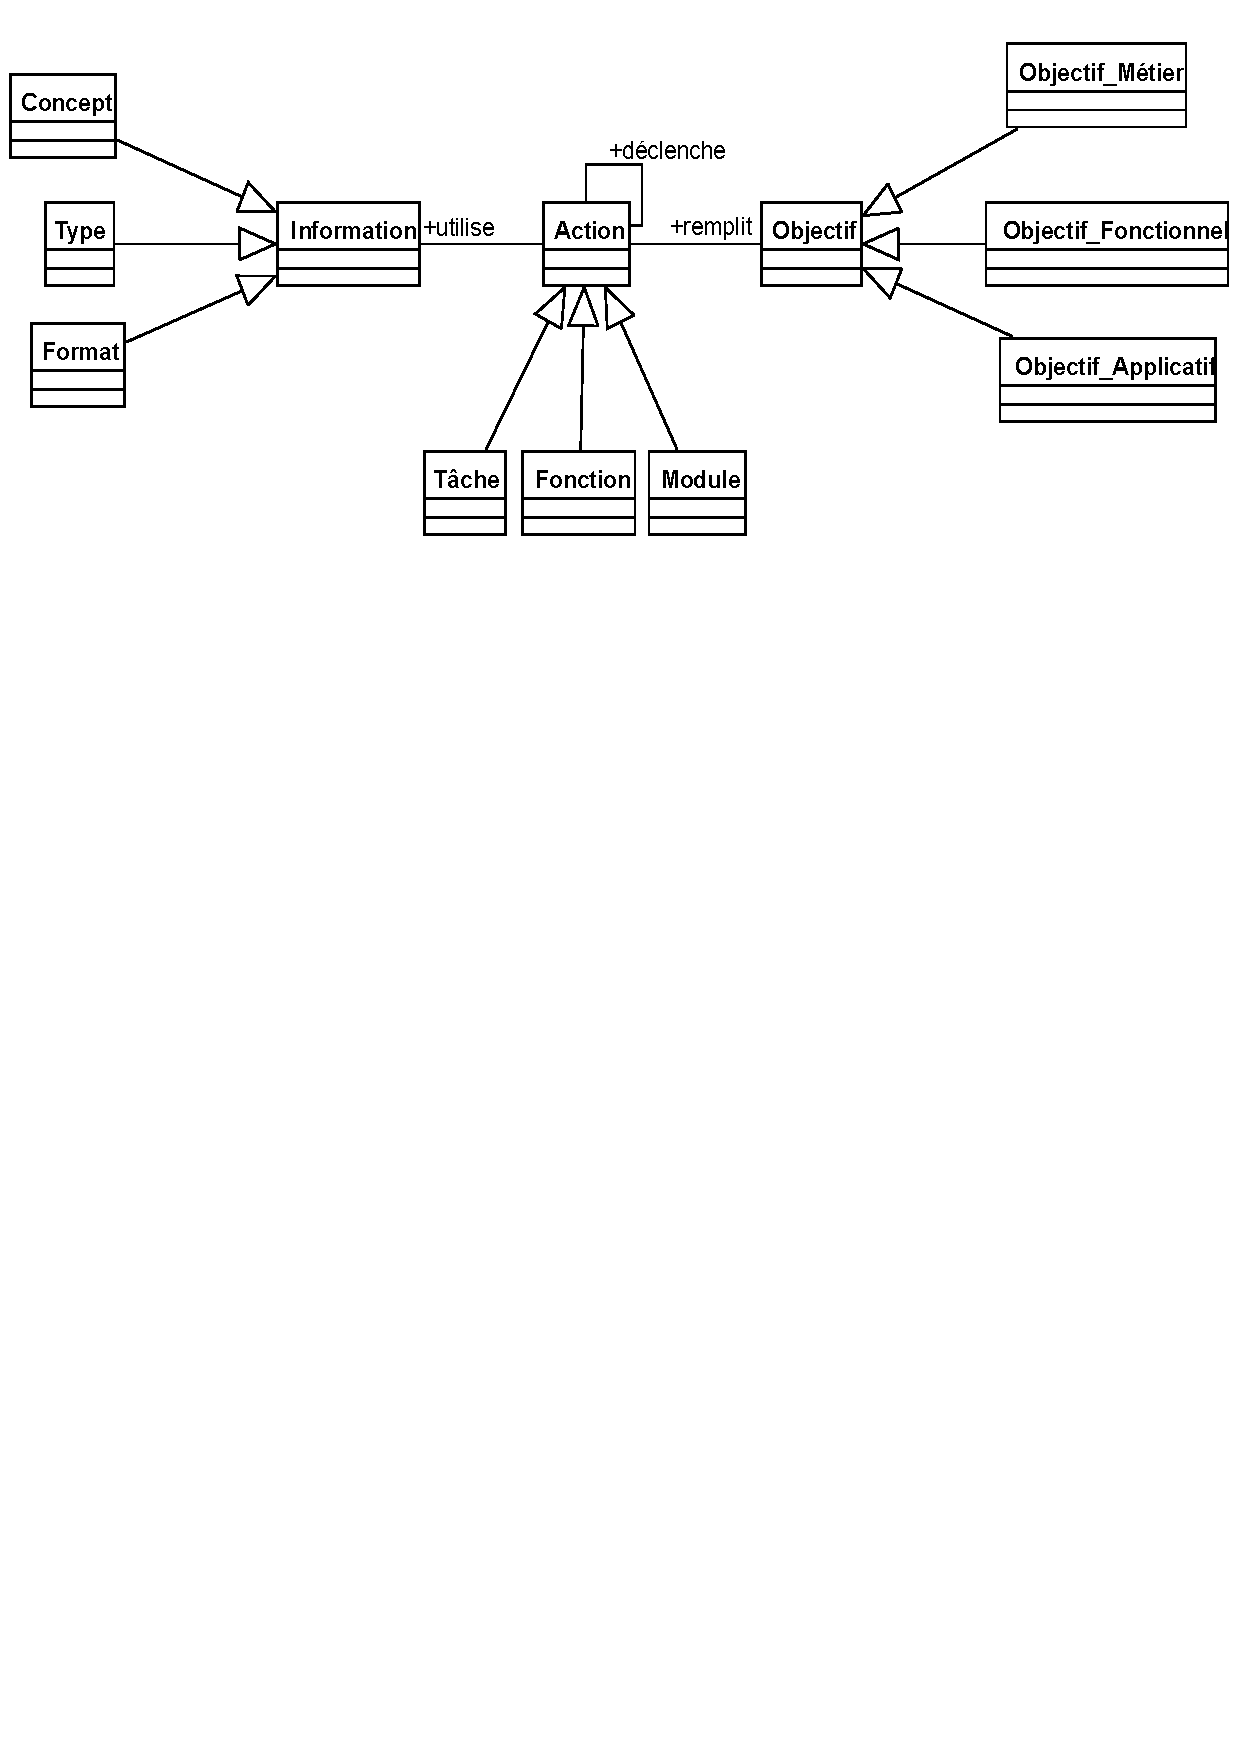
\includegraphics[trim= 0cm 20cm 0cm 0cm, width=1\textwidth]{figures/4_demarche/core_concept_vues.pdf}
        \end{center}
        \caption{Partie du métamodèle concernant la déclinaison des entités de base\\sur les vues métier, fonctionnelle et applicative} 
        \label{fig:core_concepts_vue}
    \end{figure}

Dans la partie précédente, nous présentons les éléments constitutifs à chaque vue et leurs liens de cohérence.


    \subsection{Structure globale et cohérence \emph{inter-vue}}

    La figure~\ref{fig:vue_aspect} illustre la partie du métamodèle dédiée à la représentation de la structure globale d'une architecture
    d'entreprise. Dans le métamodèle une vue peut être spécialisée en vue \q{Métier}, \q{Fonctionnelle} et \q{Applicative}. 
    Dans cette thèse, nous avons
    uniquement abordé ces trois vues tout en gardant à l'esprit la nécessité d'étendre le métamodèle la vue technique à laquelle mécanisme
    d'héritage se prête bien. Chaque vue est composée de trois aspect : \q{Information}, \q{Processus} et \q{Objectif}. 

L'aspect \q{Information} permet d'avoir un
modèle explicite des données utilisées dans chacune des vues~:

\begin{itemize} 

\item \textbf{aspect information du point de vue métier}

Cet aspect établit le modèle de données métier en regroupant les
concepts métier manipulés par le processus métier. Ce modèle est peu sujet au
changement, sauf évolution importante des pratiques métier~;
% Il est aussi à
% l'origine du découpage en bloc par entité métier de la vue fonctionnelle~;

\item \textbf{aspect information du point de vue fonctionnel}

Cet aspect établit le modèle de données fonctionnelles en regroupant les types des
données utilisées par les blocs fonctionnels nécessaires à la réalisation de
processus métier~;
% Elle décrit leurs caractéristiques et leurs relations sous
% forme de diagrammes de classes par exemple

\item \textbf{aspect information du point de vue applicatif}

Cet aspect établit le modèle de données applicatives en regroupant les formats de données
compatibles avec les modules applicatifs.

\end{itemize}

\begin{figure}[!ht]
    \begin{center}
    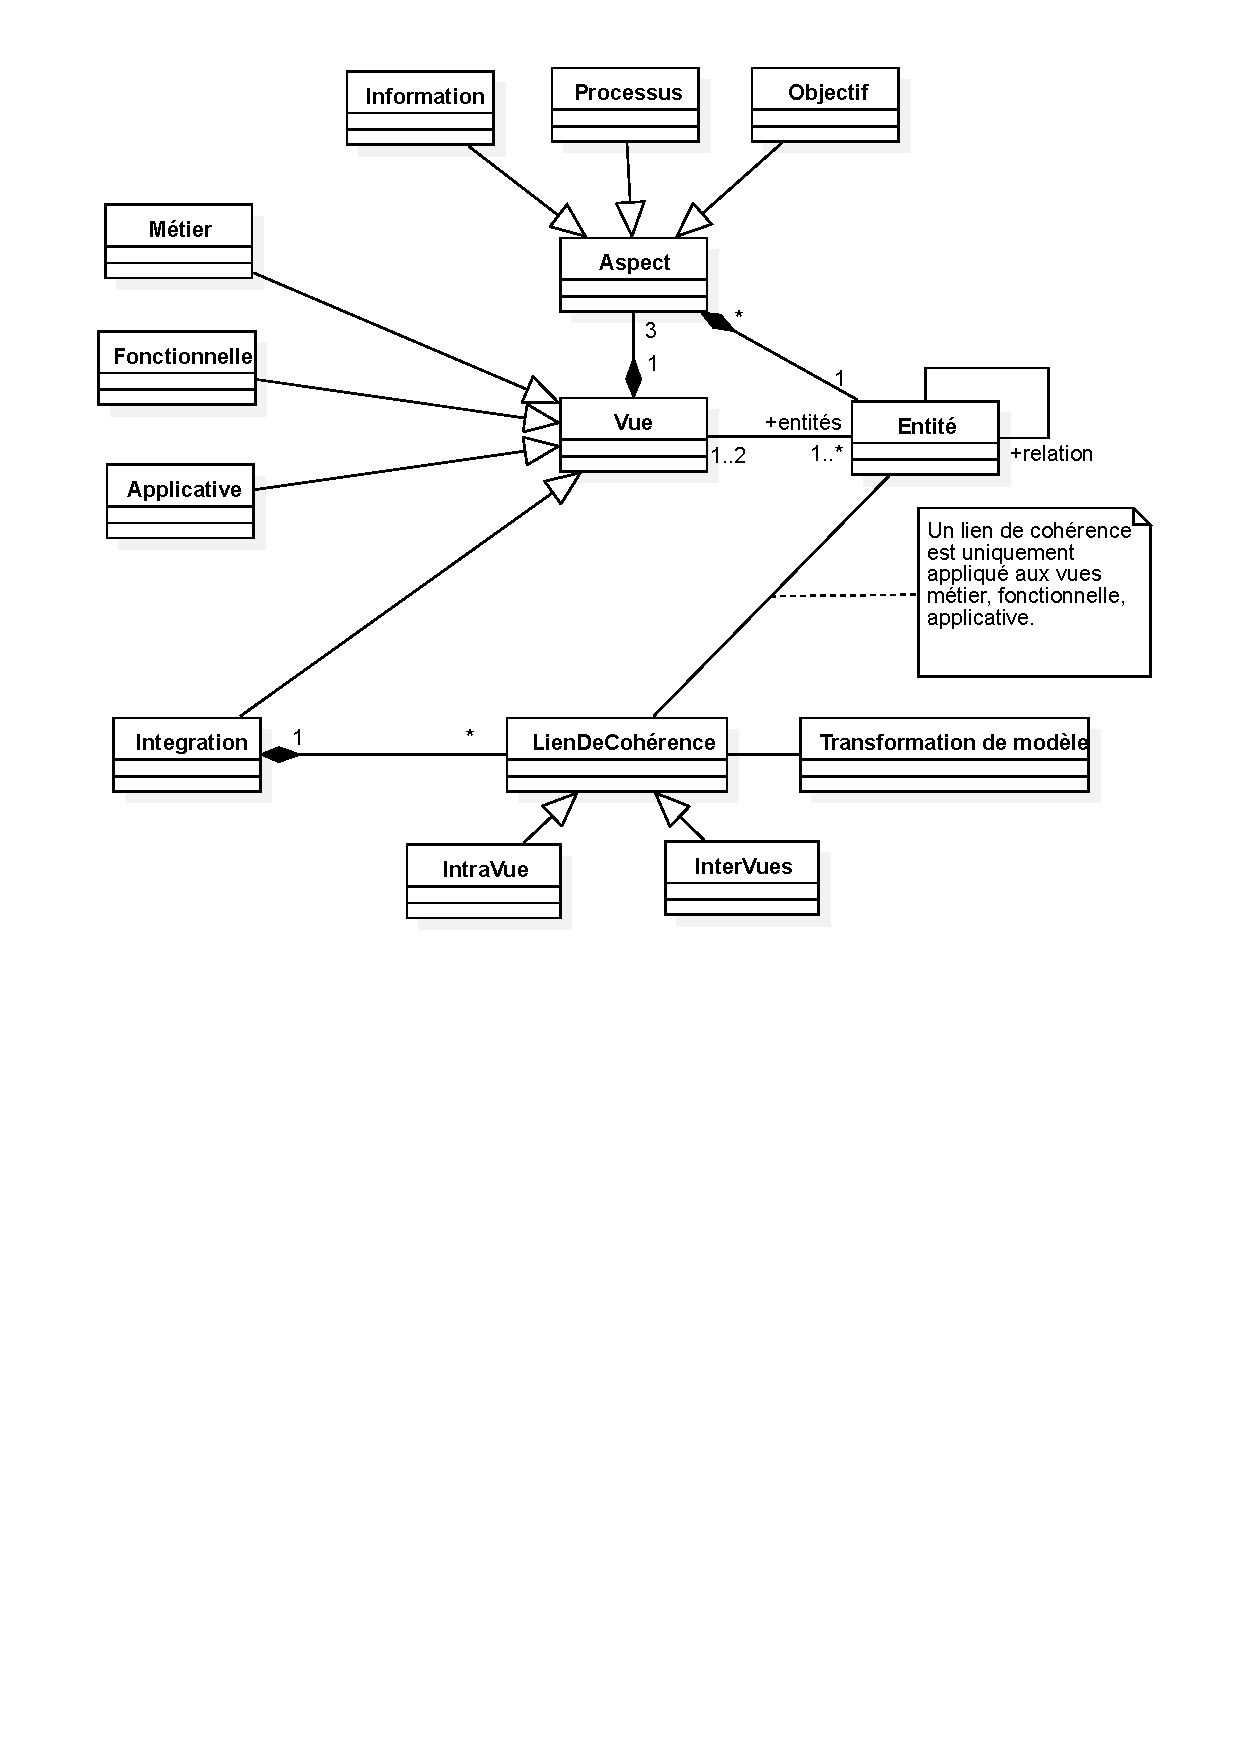
\includegraphics[trim= 0cm 14cm 0cm 0cm, width=1\textwidth]{figures/4_demarche/ea3m.pdf}
    \end{center}
    \caption{Partie du métamodèle concernant la struture globale\\d'une architecture d'entreprise} \label{fig:ea3m}
\end{figure}


De plus, nous modélisons le comportement de chaque vue dans l'aspect
\q{Processus} où un processus est constitué d'un enchaînement d'actions~:

\begin{itemize}

    \item \textbf{aspect processus du point de vue métier}

Cet aspect correspond aux processus métier de l'entreprise, décrits en termes
d’enchaînement de \q{Tâches} sans faire référence aux détails d'implémentation~;

    \item \textbf{aspect processus d'un point de vue fonctionnel}

Cet aspect correspond au processus fonctionnels de l'entreprise, décrit en termes
d'enchaînement de \q{Fonctions}~;
% qui réalisent les processus métier ainsi que
% leur orchestration en tant que processus fonctionnels. Ces fonctions sont
% regroupées en blocs. Chaque objet métier identifié dans l'aspect Information de
% la vue métier correspond à un unique bloc fonctionnel. Ceci garantit la
% construction de blocs fonctionnels fortement décorrélés, avec une forte cohésion
% interne. Dans chaque bloc fonctionnel, on retrouve les opérations correspondant
% à une tâche donnée du processus qui impacte l'objet métier impliqué~;

    \item \textbf{aspect processus du point de vue applicatif}

Cet aspect correspond au processus applicatifs de l'entreprise, décrit en termes
d'enchaînement de \q{Modules}.
% Cet aspect décrit les modules logiciels qui implémentent les blocs
% fonctionnels ainsi que leur orchestration en processus applicatifs. Dans un
% premier temps, il est conseillé de dresser un inventaire de l'existant
% applicatif et d'en extraire les modules capables de réaliser les opérations des
% blocs fonctionnels. Ensuite, si aucune application ou module existant ne peut
% répondre au besoin des nouveaux processus métier, l'architecte technique fait
% le choix des nouveaux composants applicatifs à mettre en place. En plus
% d'identifier les composants applicatifs existants ou à développer, l'architecte
% applicatif spécifie leurs interconnexions tels que échange de messages,
% synchronisation de données, transfert de fichiers périodique.

\end{itemize}

De plus, nous étendons chacune des vues par l'aspect \q{Objectif}~: 
\begin{itemize}

    \item \textbf{aspect objectif du point de vue métier}

Cet aspect regroupe les motivations métier pilotant les processus métier et modélisés
par la classe  \q{Objectif\_métier}~;

    \item \textbf{aspect objectif du point de vue fonctionnelle}

Cet aspect regroupe les motivations fonctionnelles pilotant les processus fonctionnels
et modélisés par la classe  \q{Objectif\_fonctionnel}~;

    \item \textbf{aspect objectif du point de vue applicative}

Cet aspect regroupe les motivations applicatives pilotant les processus applicatifs
et modélisés par la classe  \q{Objectif\_applicatif}.

\end{itemize}

% D'une part, modéliser cet aspect permet de garder
% une traçabilité d'une entre les processus modélisés et les objectifs qu'ils sont
% censés remplir. D'autre part, il permet de décliner les objectifs métier en
% objectifs applicatifs, et les objectifs applicatifs en objectifs fonctionnels.
% Comme nos travaux adoptent l'école de pensée «~Architecture du Système
% Entreprise~», nous souhaitons évaluer non seulement la composante SI mais également
% l'ensemble de l'entreprise. L'aspect objectif est un moyen de
% modéliser explicitement la stratégie de l'entreprise, traduite en un ensemble
% cohérent d'objectifs métier et ce pour évaluer la capacité des processus mis en
% place à y répondre et pour évaluer la stratégie elle-même par rapport à la
% réalité de l'entreprise.

La préoccupation majeure de l'EA réside dans l'alignement métier/IT \cite{kaisler_enterprise_2005},
c'est-à-dire l'alignement d'un même aspect entre deux vues d'architecture différentes.
Nous proposons est d'y dédier une vue spécifique~: la vue intégration.
Ainsi, en plus d'expliciter les liens de cohérence à l'intérieure d'une même vue
à travers la classe \q{IntraVue} abordée dans la section
~\ref{sec:intravue}, la vue intégration permet de modéliser les liens de traçabilité
entre des éléments relatifs à un même aspect et appartenant à des vues différentes en spécifiant les relations de
raffinement à travers la classe \q{InterVues} du métamodèle.
 
 La figure~\ref{fig:metamodele_vue_integration} illustre la partie du métamodèle dédiée à la vue intégration.
 En plus des liens de cohérence intra-vue, nous y modélisons les liens de cohérence
 inter-vues à travers la relation \q{raffine}. Ainsi, une tâche est raffinée par une ou
 plusieurs fonctions qui la réalisent, elles-mêmes raffinées par un ou plusieurs modules applicatifs
 qui les implémentent. De même, un objectif métier est raffiné par un ou plusieurs objectifs fonctionnels,
 eux-mêmes raffinés par un ou plusieurs objectifs applicatifs. De manière analogue, un concept métier est raffiné
 par un ou plusieurs types fonctionnels, eux-mêmes raffinés par un ou plusieurs formats applicatifs.

\begin{figure}[!ht] \begin{center}
    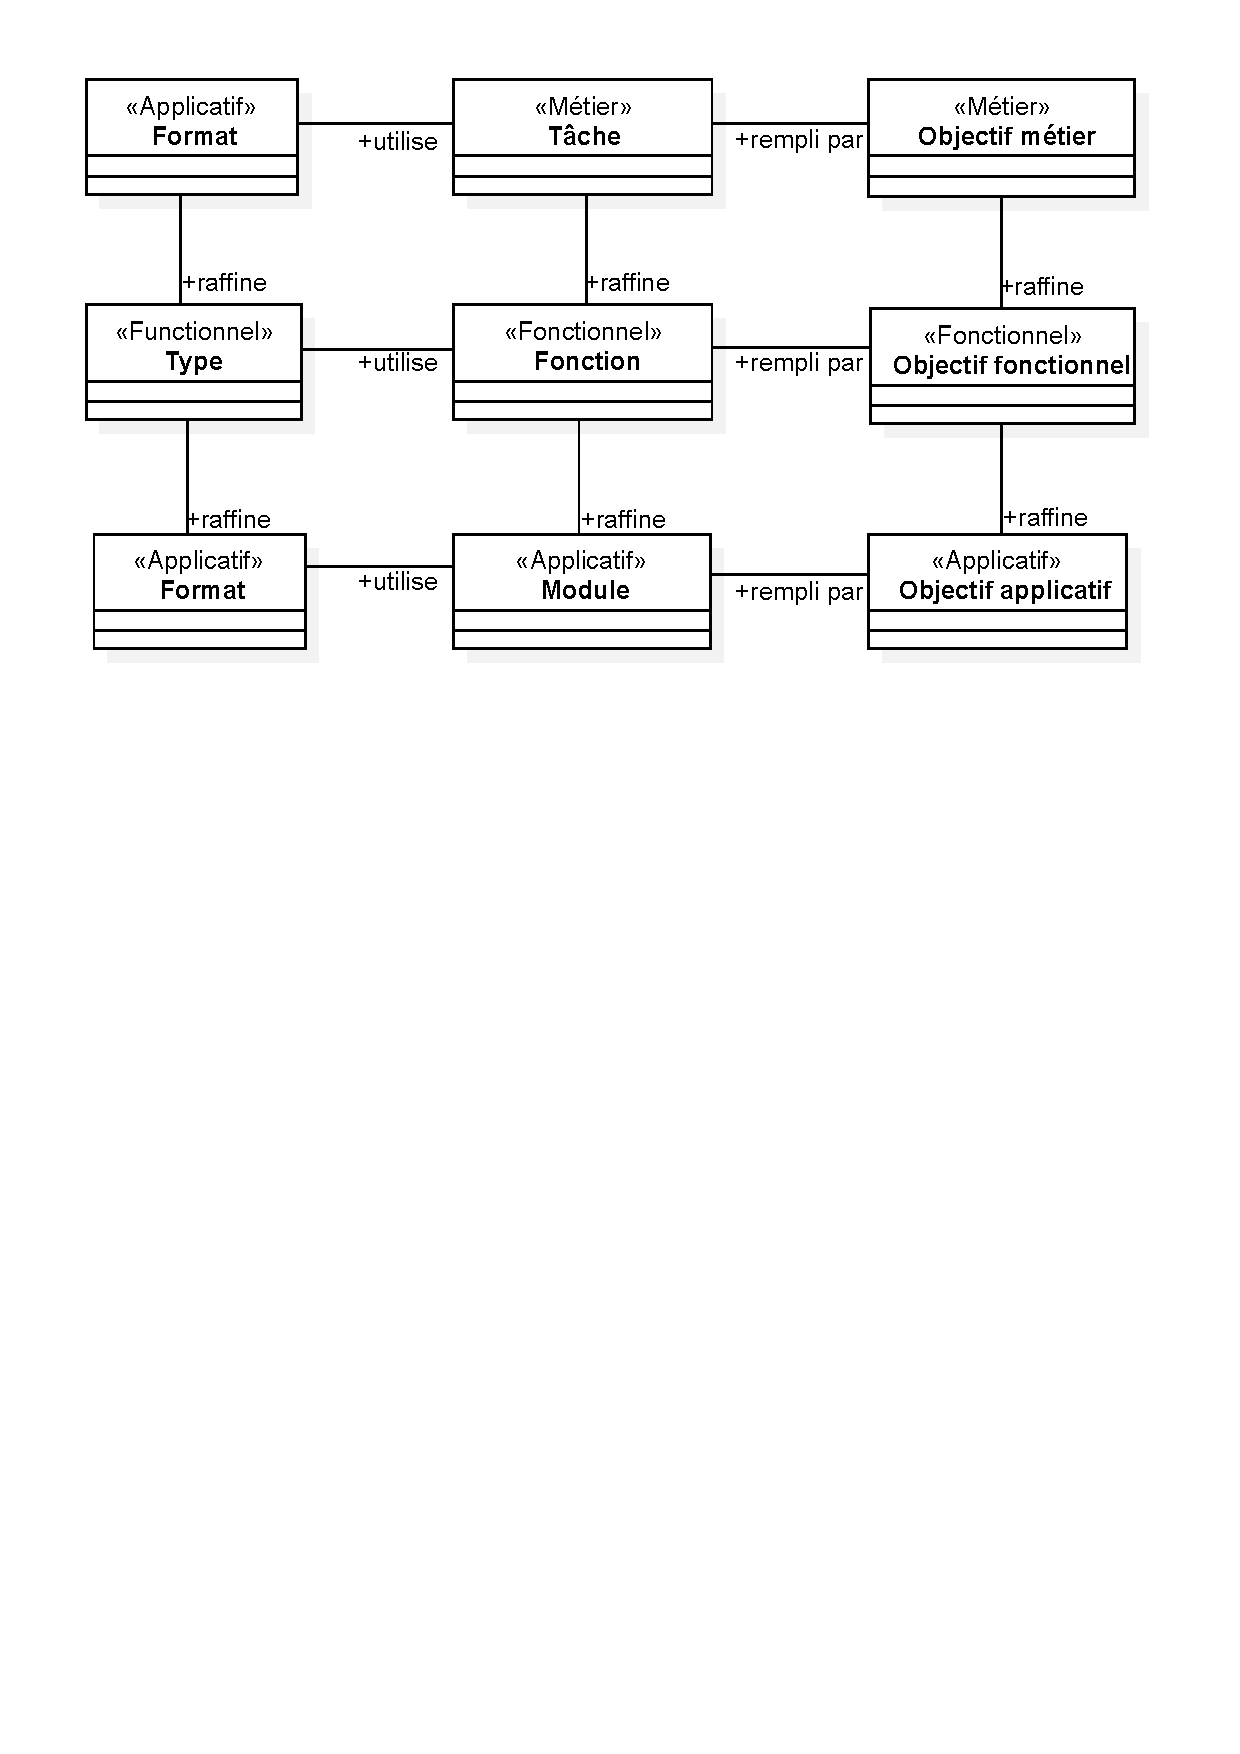
\includegraphics[trim= 0cm 18cm 0cm 0cm, width=1\textwidth]{figures/4_demarche/metamodele_vue_integration.pdf}
    \end{center}
    \caption{Métamodèle de la vue intégration}
    \label{fig:metamodele_vue_integration}
\end{figure}


Qu'il s’agisse d'une cohérence intra-vue ou inter-vues, la vue intégration définit un \textit{mapping} en spécifiant
(1)~les entités à aligner, (2)~les liens de cohérence entre ces éléments et (3) des transformations de modèle
associées à ces liens. Nous identifions plusieurs cas de figures où ces transformations de modèle s'avèrent commodes
dans le contexte de l'EA dans la section \ref{sec:executeea}. Parmi ces cas de figure nous citons, notamment,
l'automatisent du passage d'une vue à l'autre en utilisant une transformation de modèle pour générer le code
d'un module de la vue applicative à partir d'un modèle de fonction de la vue fonctionnel.

\section[Le framework ExecuteEA]{Le \emph{framework} \emph{ExecuteEA}}
\label{sec:executeea}
    
    % framework = approche conceptuelle + structure logique (pour organiser et mettre en cohérence les modèles d'architecture  + outils et langages

    Une approche par points de vue est indispensable à l’appréhension des systèmes complexes car elle permet de séparer
    les préoccupations des parties-prenantesdans des vue distinctes. Chaque vue traduit donc la perspective d'une partie-prenante.
    De nombreux \emph{frameworks} d'EA adoptent de ce fait une approche par points de vue. Cependant, les différentes préoccupations
    sont souvent traitées de manière séquentielle et plus ou moins indépendante des autres vues comme l'attestent
    S.~Kurpjuweit et R.~Winter~\cite{kurpjuweit2007viewpoint}.

    Nous proposons donc un \emph{framewok} d'EA permettant de traiter
    les différentes vues d'architecture de manière intégrée tout en permettant à l'architecture d'entreprise d'accompagner l'entreprise
    sur toute sa trajectoire.  Le métamodèle EA2M représente la pierre angulaire de ce \emph{framework}.
    Nous recourons en effet à la méta-modélisation pour unifier les différentes activités
    d'architecture —~documentation, analyse et conception~—
    en les inscrivant dans le cadre méthodologique et technologique offert par l'IDM.

    La vision unificatrice de l'IDM a pour \emph{leitmotiv} l'usage systématique de modèles productifs~\cite{2005unification}, c'est-à-dire
    de modèles \textbf{exécutables} \emph{versus} les modèles purement contemplatifs habituellement utilisés pour mener 
    pour les différentes activités d'EA~\cite{kulkarni2013modelling}. Nous avons donc choisi la dénomination \emph{Execute Enterprise Architecture} (\emph{ExecuteEA}) pour le \emph{framework} que nous présentons dans cette section.

    Le \emph{framework ExecuteEA} repose sur trois piliers~: (1)~une approche unificatrice pour la modélisation d'architecture d'entreprise,
    (2)~un cadre structurant orienté points de vue et (3)~l'identification d'un ensemble de langages et de techniques issus de l'IDM
    et adaptés à l'analyse d'architecture d'entreprise.



    % L'IDM prône en effet le recours systématique aux modèles productifs sur toute la chaine de production d'u 
    % Dans ces travaux de thèse, nous adoptons l'école de pensée \emph{Enterprise System Architecting} telle que définie
    % par Lapalme~\cite{lapalme2012three} et présenté dans le chapitre~\ref{ch:EA} traitant de l'état de l'art du domaine de l'EA.
    % De nombreux travaux ont démontré la capacité de l'IDM à traiter la complexité inhérente aux systèmes logicielles dont notamment
    % ceux de R. France et et B. Rumpe~\cite{france2007model}.


   \subsection{Approche conceptuelle et cadre structurant}

Parmi les différentes activités d'EA, nous avons choisi de focaliser nos travaux de thèse sur l'activité
d'analyse et ce pour plusieurs raisons.

D'abord, l'analyse fait partie des activités les moins traitées en EA~\cite{chen2008architectures} \cite{barn2013enterprise},
quelle qu'en soit l'école de pensée comme relaté dans l'état 
de l'art concernant l'EA présenté au chapitre~\ref{ch:EA}. Cet état de fait est en partie du
aux limitations des modèles contemplatifs qui font légion en EA. C'est pendant l'activité l'analyse que les modèles
exécutables sont le plus valorisés et indispensables.

Ensuite, comme l'illustre la figure~\ref{fig:activite_ea} l'analyse joue un rôle central dans une démarche d'EA.
Les modèles issus de l'analyse peuvent directement servir à documenter l'EA (\q{modèles EA validés} dans la figure~\ref{fig:activite_ea}).
Il s'agit de modèles qui recourent directement aux concepts du domaine de l'EA 
et qui ne nécessitent donc pas de changer de niveau d'abstraction pour être appréhendés par les parties-prenants.
En IDM, ces modèles sont qualifiés de \emph{problem-level abstration models} \cite{france2007model}.

\begin{figure}[!ht] \begin{center}
    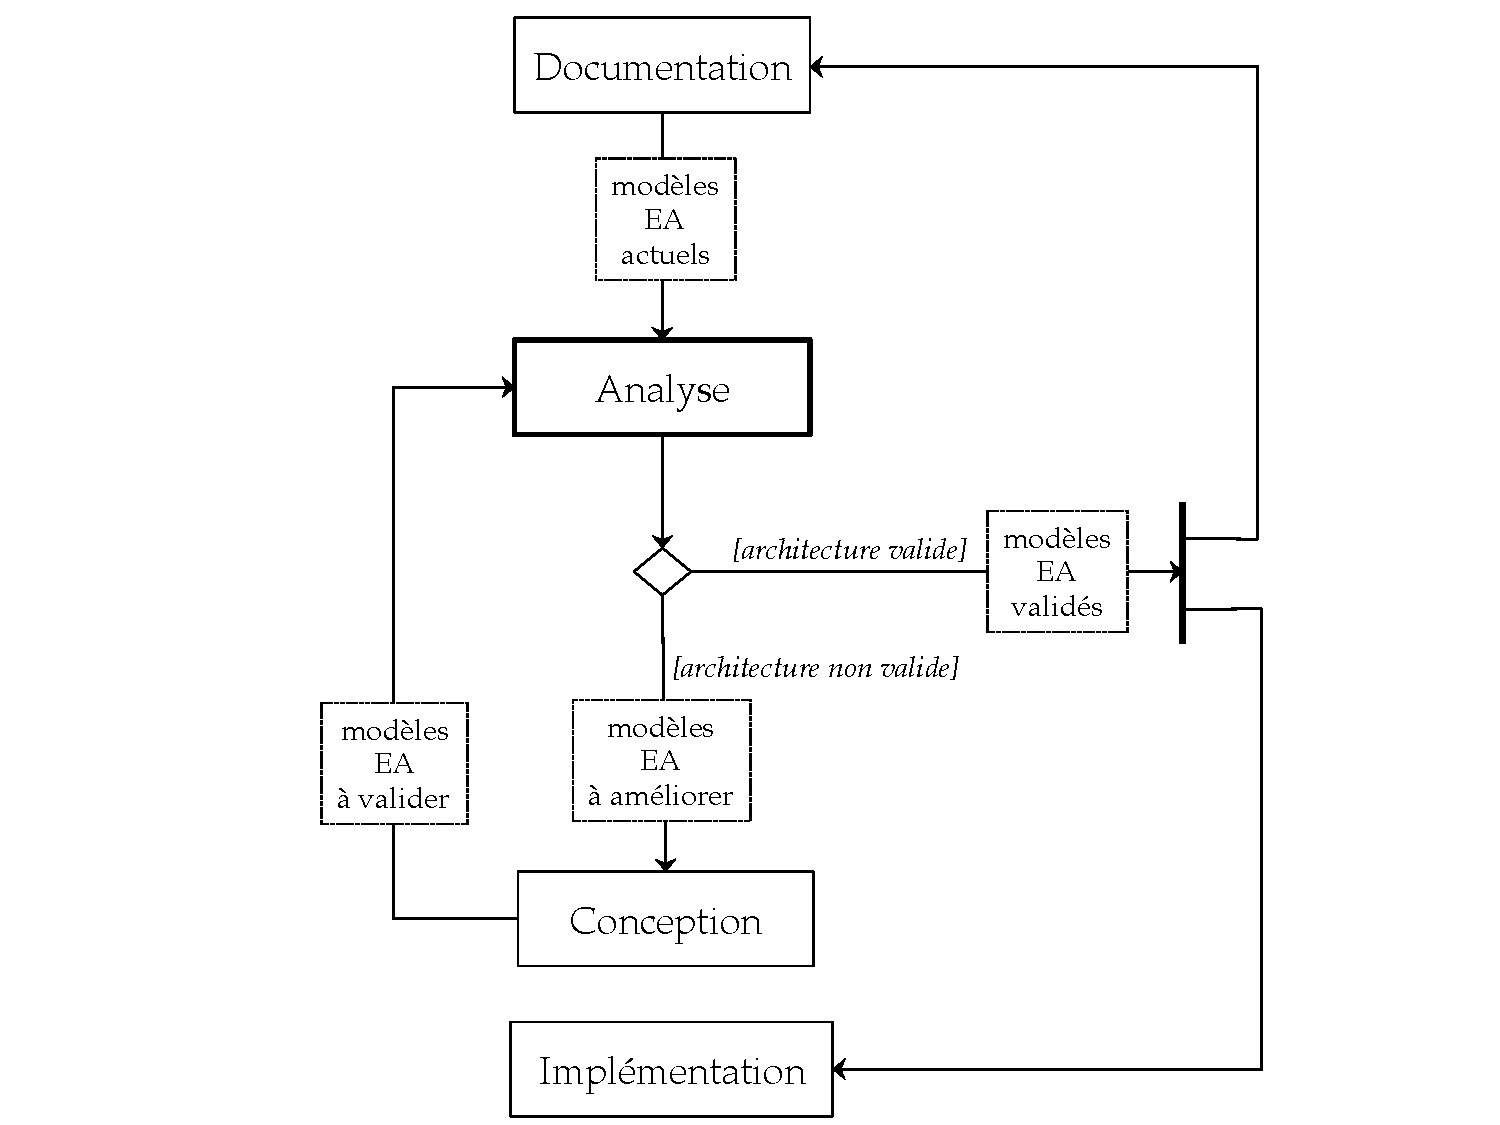
\includegraphics[width=1\textwidth]{figures/4_demarche/activite_ea.pdf}
    \end{center}
    \caption{Évolution des modèles d'architecture\\et rôle central de l'activité d'analyse en EA}
    \label{fig:activite_ea}
\end{figure}

Enfin, l'analyse de modèles d'architecture est fortement liée à l'activité de conception. Le recours aux modèles
exécutables pour la conception d'architecture d'entreprise permet de mener des analyses directement sur ces
même modèles (\q{modèles EA à améliorer} et \q{modèles EA à valider} dans la figure~\ref{fig:activite_ea}). Dès lors que ces modèles sont validés à l'issue des activités d'analyse et de conception,
il devient possible de les utiliser à pour la documentation (en mettant
automatiquement à jour les anciens modèles d'architecture) et pour l'implémentation. L'implémentation peut 
alors se faire par transformation de modèles, en transformant les \q{modèles EA validés} vers la plate-forme cible.

Nous entendons analyser deux aspects distincts mais corrélés d'une architecture
d'entreprise~: la structure et le comportement de la dite architecture.
L'analyse de la structure repose essentiellement sur la formalisation du métamodèle EA2M et vise à 
intégrer des modèles provenant des différentes vues d'architecture afin de garantir la cohérence
de l'ensemble de l'architecture. L'analyse du comportement de l'architecture repose quant à elle
essentiellement sur la simulation des modèles issus de l'analyse de la structure.
%Nous détaillons les activités l'analyse de la structure et du comportement dans la section~\ref{sec:analyse}.

\begin{figure}[!ht]
 \begin{center}
 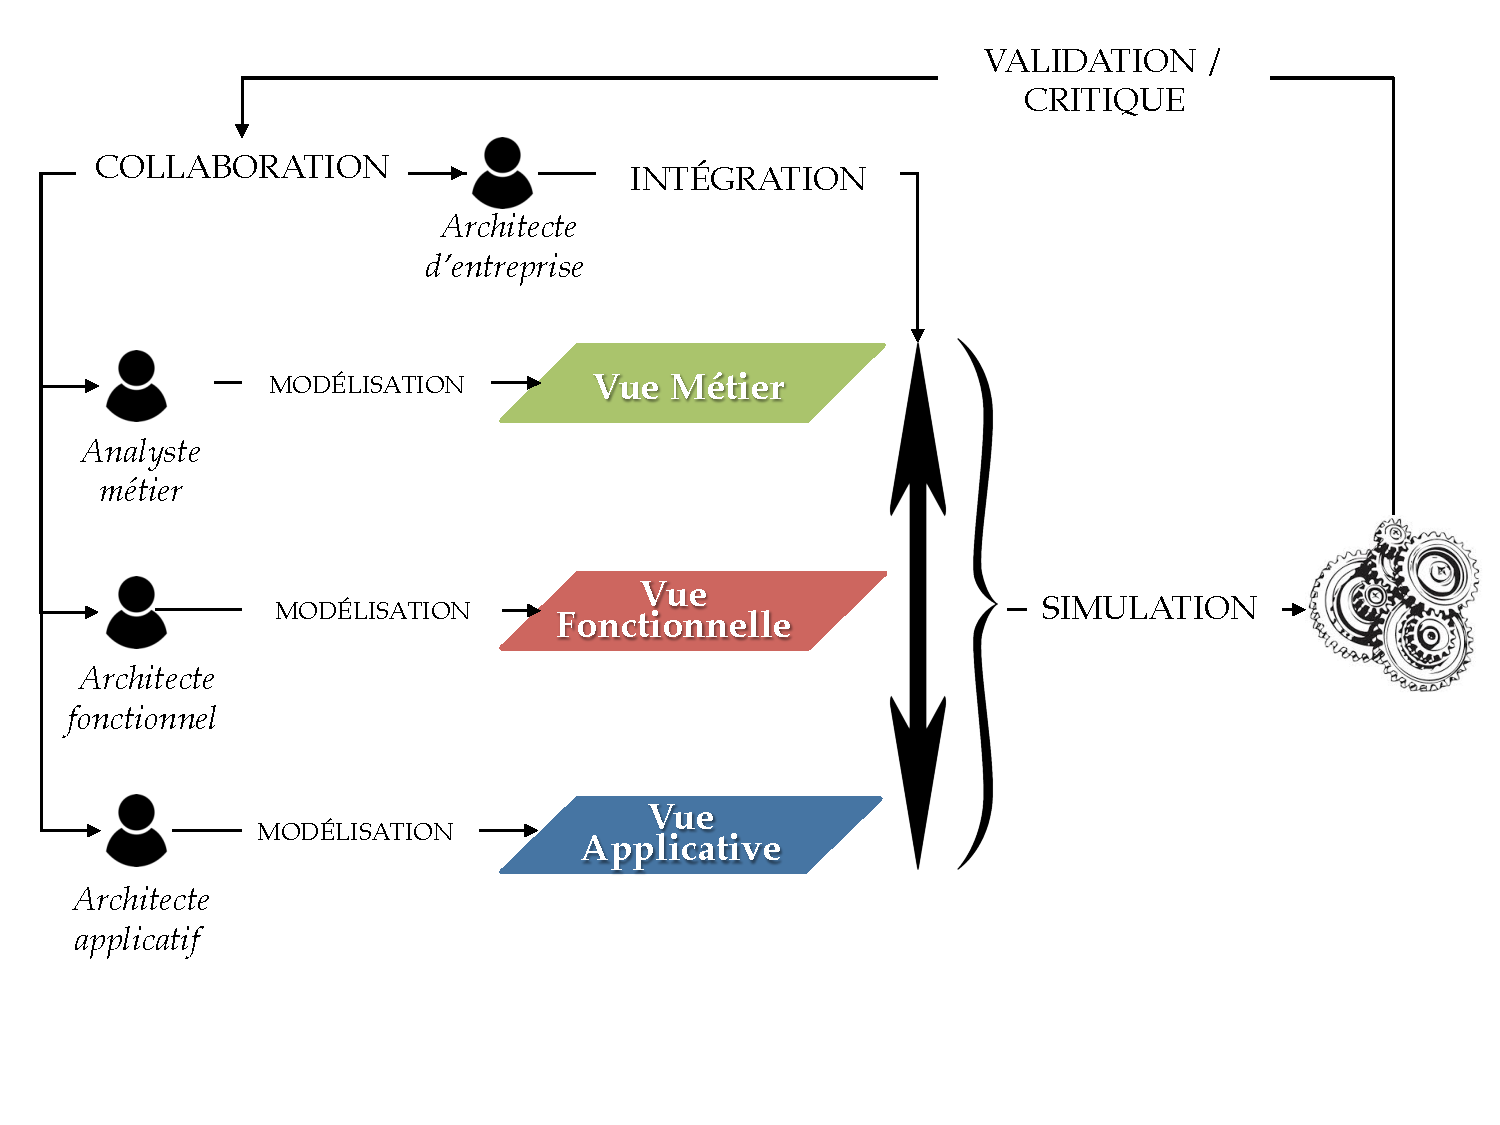
\includegraphics[trim= 0cm 2.5cm 0cm 0cm, width=1\textwidth]{figures/4_demarche/approche_conceptuelle.pdf} \end{center}
 \caption{Approche conceptuelle du \protect\emph{famework ExecuteEA}}
 \label{fig:approche_conceptuelle}
\end{figure}

Le \emph{framework ExecuteEA} englobe une approche conceptuelle et un cadre structurant les différentes activités d'EA, dont
notamment  l'analyse. Nous commençons par présenter l'approche conceptuelle illustrée par la figure~\ref{fig:approche_conceptuelle}.
L'approche consiste à définir un processus précis en identifiant
quatre rôles participant à ce processus~: l'architecte métier,
l'architecte fonctionnel, l'architecte applicatif et enfin l'architecte d'entreprise. Les trois premiers rôles ont déjà été présentés
dans la section~\ref{sec:roles}. 



Le processus commence par la modélisation de la vue métier par l'architecture
métier. L'architecte fonctionnel traduit la vue métier en une vue fonctionnelle 
en collaborant avec l'architecte
métier. L'architecte applicatif traduit la vue fonctionnelle en une vue applicative
tout en collaborant avec l'architecte fonctionnel et par extension avec l'architecte
métier. Le rôle de l'architecte d'entreprise consiste alors à orchestrer l'ensemble de ces
collaborations.

L'architecture ainsi modélisée est soumise à une analyse
structurelle menée par l'architecte d'entreprise en étroite collaboration avec
les architectes des différentes vues. L'architecte d'entreprise est alors
responsable de la vue intégration qui a pour mission de vérifier la cohérence
globales des modèles d'architecture. Ainsi intégrés, les modèles sont soumis à
une analyse comportementale via la simulation.
L'approche proposée suit un processus itératif. À l'issue de la simulation, l'ensemble des
architectes valident ou modifient leurs modèles selon les résultats de la simulation et ainsi de
suite jusqu'à obtenir une architecture satisfaisante pour l'ensemble des parties-prenantes.

\begin{figure}[!ht]
 \begin{center}
 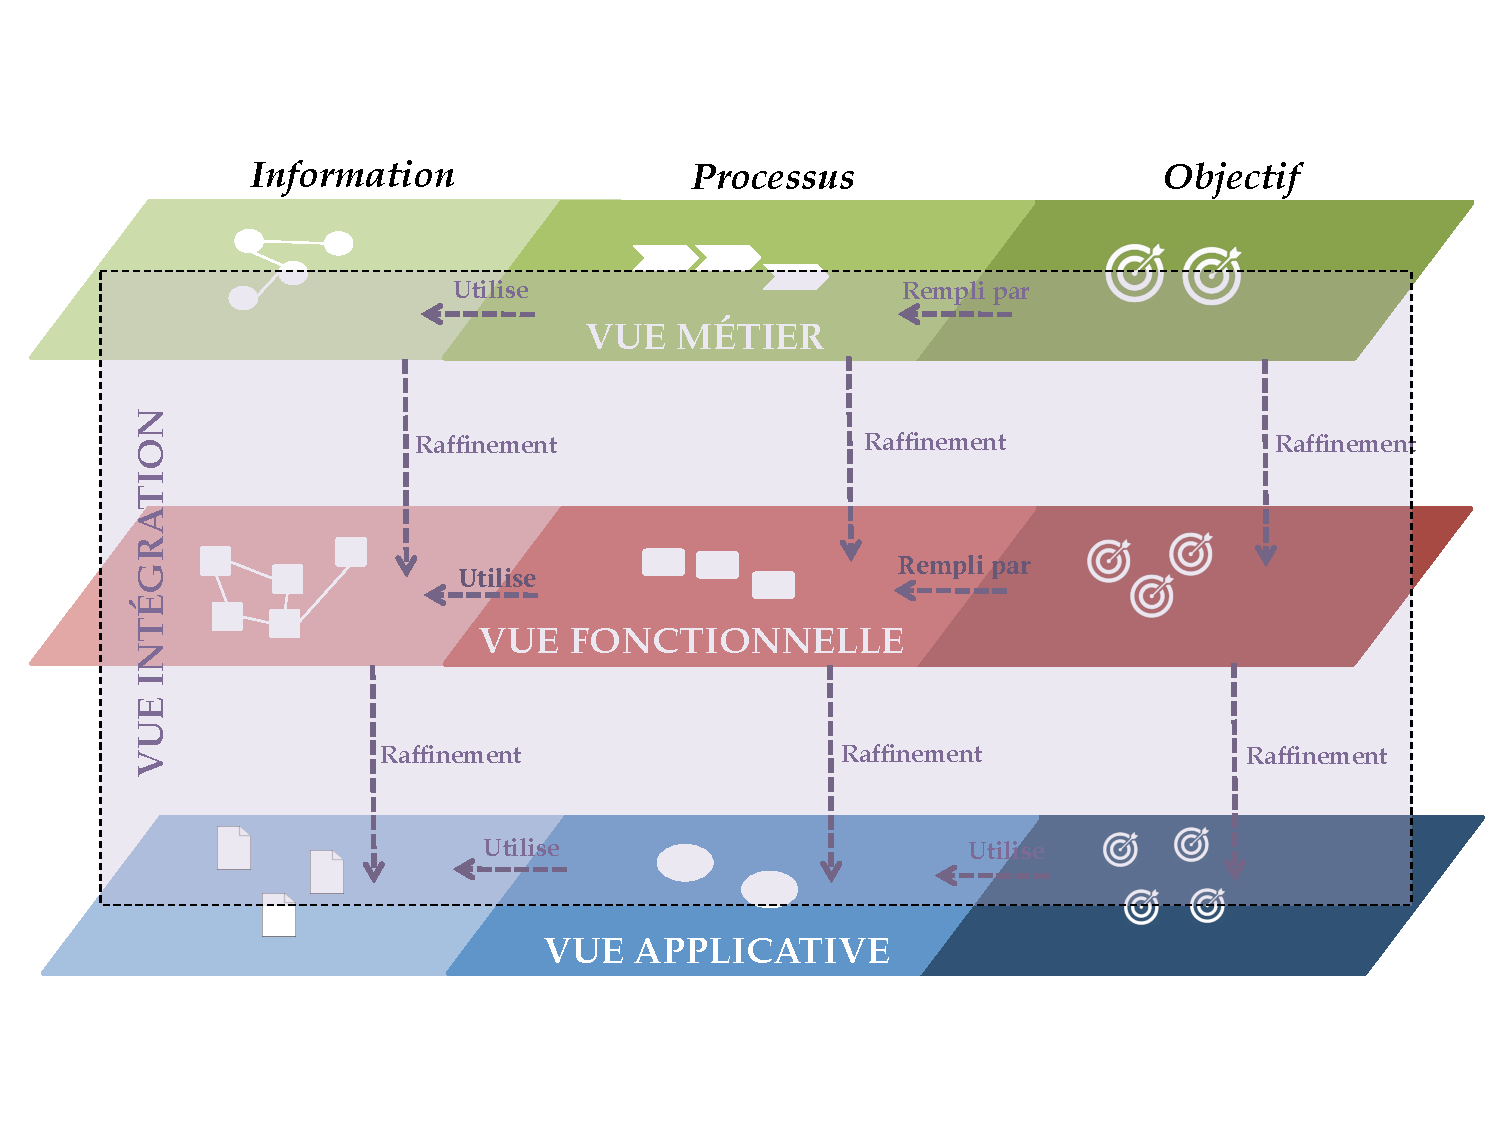
\includegraphics[trim= 0cm 2cm 0cm 0cm, width=1\textwidth]{figures/4_demarche/vue_integration.pdf}
 \end{center}
 \caption{Cadre structurant de \protect\emph{ExecuteEA}}
 \label{fig:vue_integration}
\end{figure}

L'approche proposée s'inscrit en outre dans un cadre structurant qui reprend les concepts identifiés dans le métamodèle
EA2M. Ce cadre est illustré par la figure~\ref{fig:vue_integration}. Ce cadre structure et organise les différents modèles
créés par les architectes~: métier, fonctionnel et applicatif. Chaque vue est en effet composant de trois aspects~: information,
processus et objectif. Notre contribution principale consiste à doter ce cadre d'une vue intégration transverse à toutes les autres vues.
Cette vue reflète la perspective de l'architecte d'entreprise qui a pour mission de garantir la cohérence globale de l'architecture
et s'assure de l'alignement métier/IT. La vue intégration permet donc à l’architecte d'entreprise
d'expliciter les liens de cohérence intra-vue (\emph{via} les liens \q{remplit} et \q{utilise}) et inter-vues (via les liens de \q{raffinement}).




% Créer des modèles d'architecture d'entreprise qui sont appropriés à l'analyse des 
% modèles d'architecture implique de suivre un processus précis. 
% L'objectif de nos travaux est de définir le processus de modélisation approprié, les
% rôles impliqués, les artefacts conceptuels requis, ainsi que les outils et les
% langages adéquats pour mener des analyses de structure et de comportement.

% Notre contribution est double. Tout d'abord, nous proposons un frune démarche de
% modélisation et d'analyse qui s'appuie sur un cadre d'architecture multi-vues.
% Nous dotons ce cadre d'architecture d'une vue supplémentaire qui est la vue
% \textit{intégration}. Cette vue a pour but d'adresser les problématiques de
% cohérence et d'alignement. Ensuite, nous mettons à profit les langages et
% standards de l'IDM permettant de modéliser et de simuler les architectures
% d'entreprise.




% \begin{figure}[!ht]
%  \begin{center}
%  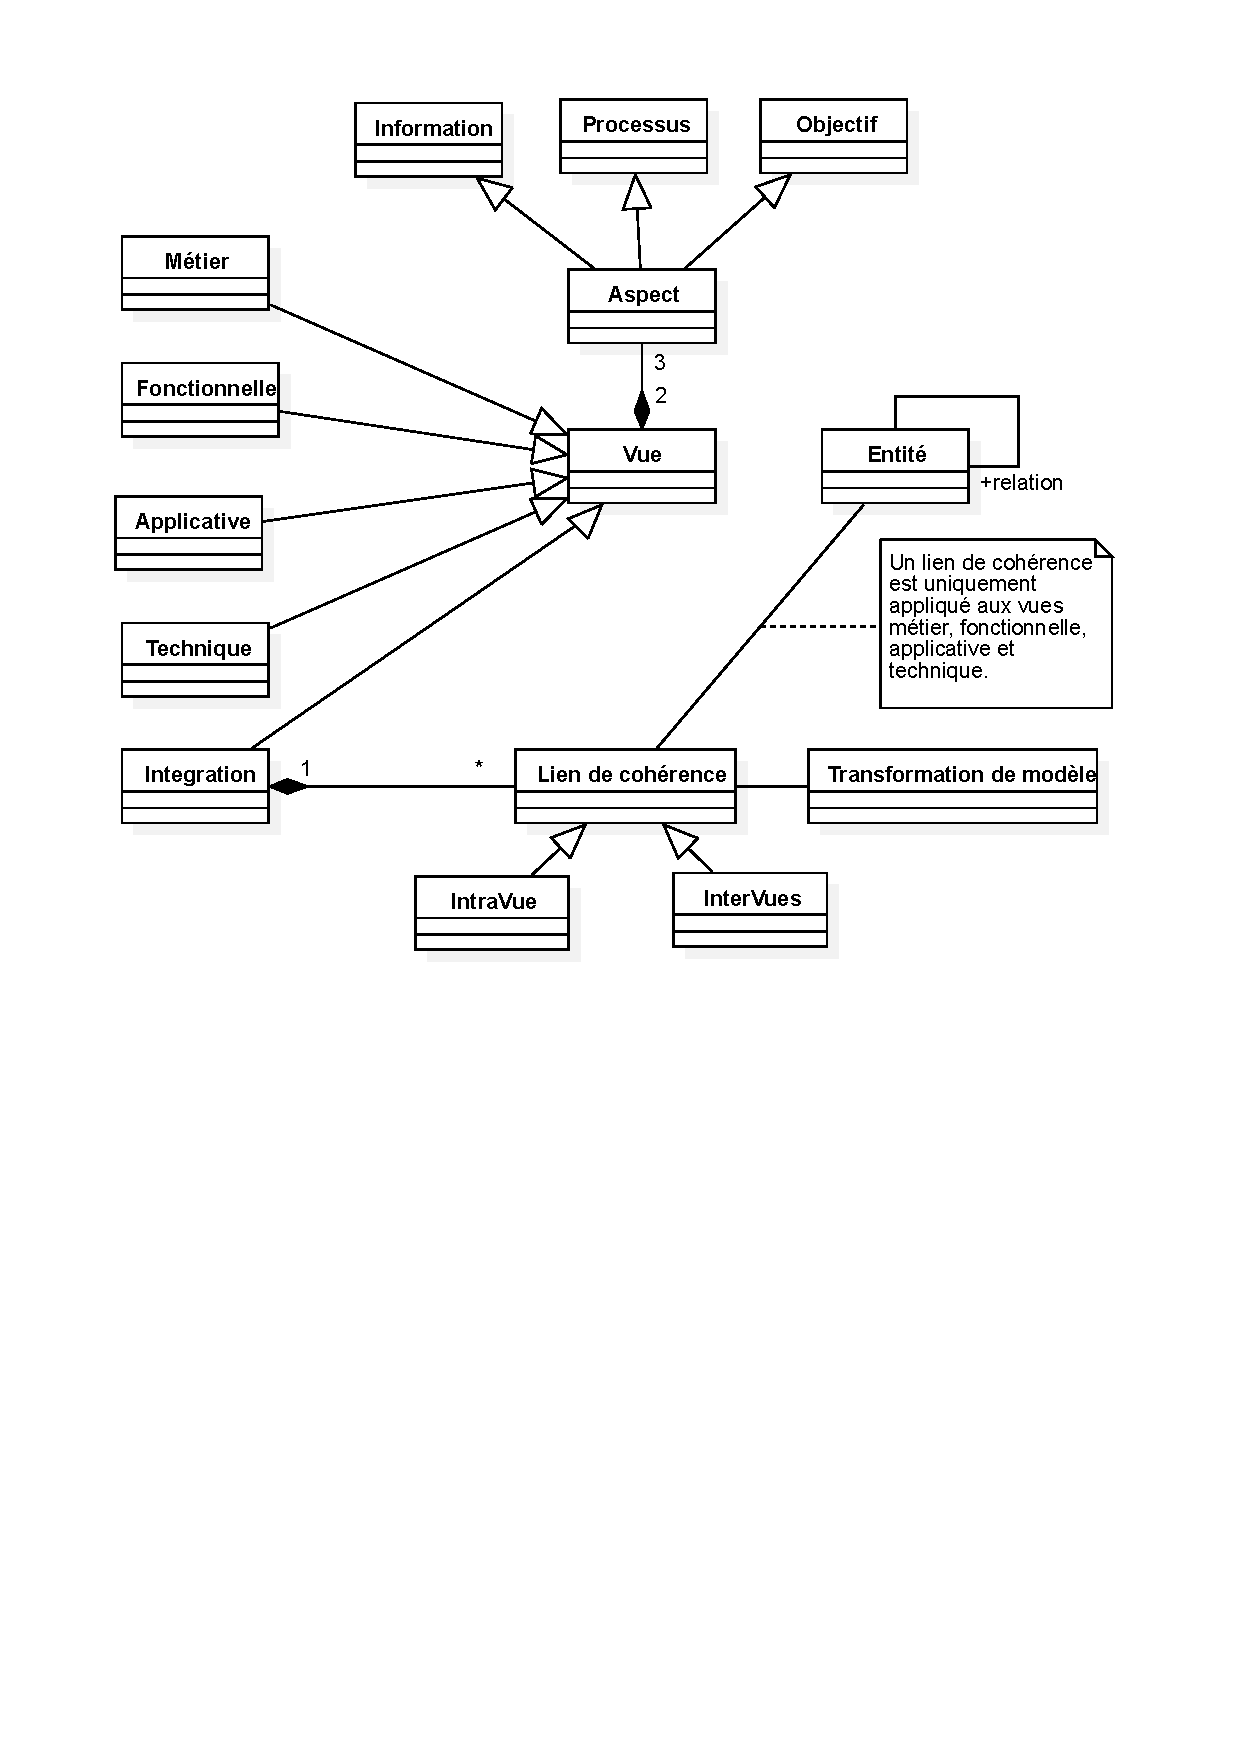
\includegraphics[trim= 0cm 13cm 0cm 2cm, width=1\textwidth]{figures/4_demarche/metamodele_framework.pdf} \end{center}
%  \caption{Métamodèle du framework proposé}
%  \label{fig:metamodele_framework}
% \end{figure}

% Nous donnons le métamodèle de la vue intégration dans la figure
% \ref{fig:metamodele_vue_integration}. Cette vue permet des vérifications
% horizontales à l'intérieur de chacune des vues. En effet, l'association
% «~utilise~» assure donc la compatibilité des données échangées entre les tâches
% d'un processus métier, les fonctions d'un bloc fonctionnel ou entre les modules
% d'une application (voir figure \ref{fig:metamodele_vue_integration}).
% L'association «~rempli par~» hérite aussi de la classe «~IntraVue~» et associe
% explicitement une entité à l'objectif qui lui est assigné. De cette manière, il
% est possible de tracer l'implémentation effective d'une stratégie métier à
% travers l'ensemble de l'entreprise, des entités métier à l'IT.




% Nous considérons donc que la documentation et la communication, l'analyse et la
% compréhension et enfin la conception et l'implémentation concernent tout le système entreprise et
% pas seulement sa composante SI. Par exemple, contrairement à une EA centrée sur
% les SI, les processus métier sont modélisés et évalués tout autant que
% l'architecture applicative. 



% L'analyste métier, l'architecte fonctionnel et l'architecte applicatif
% collaborent entre eux et avec l'architecture d'entreprise pendant tout le
% processus de modélisation. Par la suite, l'activité d'intégration incombe à
% l'architecte d'entreprise, détenteur de la vision globale. Mais l'intégration
% des vues implique de rebouclage avec les autres acteurs (analyste métier,
% architecte fonctionnel et architecte applicatif) pour garantir l'alignement
% business/IT. Les étapes de modélisation et d'intégration de notre approche
% répondent donc aux objectifs de conception et de communication tels que définis
% par Kurpjuweit et Winter \cite{kurpjuweit2007viewpoint}.




    \subsection{Analyse de l'architecture d'entreprise}
    \label{sec:analyse}
Le cadre structurant et l'approche conceptuelle du \emph{framework ExecuteEA} permettent de mieux articuler entre elles les activités d'analyse de la structure et du comportement. L'analyse automatisée de ces modèles facilite leur appréhension par l'acteur qui
mène ces analyses (en l'occurrence l'architecte d'entreprise). Dans cette section, nous expliquons comment le recours aux modèles exécutables tel que préconisé par l'IDM permet de réaliser ces analyses.

    \subsubsection{Analyse de la structure}


L'analyse structurelle d'une architecture d'entreprise a plusieurs visée. Il peut s'agir de (1) la
vérification de la cohérence de l'ensemble de l'architecture (2) anticiper les changements en
en mesurant par exemple l'impact du changement \cite{de2005change} sur la structure de l'architecture.
Le métamodèle EA2M rend possible cette analyse en exploitant la relation de conformité qui lie un modèle à son
métamodèle telle que présentée dans l'état de l'art concernant les relations de base de l'IDM
au chapitre~\ref{ch:IDM}. 

La formalisation d'un métamodèle pour l'EA permet de plus de
contrôler la conformité des modèles d'architecture. En effet, le métamodèle
contraint les modèles d'architecture et offre la possibilité de vérifier
que l'ensemble des modèles respectes bien les contraintes exprimées par le
métamodèle.
Dans le cadre de EA2M, ces contraintes sont exprimés à travers les liens
de cohérence. Par exemple, toutes les entités de base (action, objectif et information)
doivent toujours appartenir à deux vues~: la vue intégration en plus d'une autre vue
parmi les vues métier, fonctionnelle, applicative et technique. Cette contrainte permet de vérifier
que toutes les entités de l'architecture sont bien répertoriées dans la vue intégration.

Autre exemple de contraintes exprimées dans le métamodèle EA2M~: tous les objectifs de la vue métier
doivent avoir des liens de cohérence inter-vues avec les objectifs de la vue fonctionnelle, et de même pour ces dernier
avec les objectifs de la vue applicative. Cette contrainte permet de vérifier que tous les objectifs exprimés par le métier sont bien pris
en compte par les applications de l'entreprise. Cette cohérence inter-vues est renforcée par une autre contrainte intra-vue
exprimée dans le métamodèle EA2M. Chaque action doit disposer d'un lien de traçabilité vers l'objectif qu'elle remplit.
Le croisement  de ces deux contraintes, exprimées au niveau du métamodèle, permet de vérifier que les modèles disposent
bien des liens de traçabilité nécessaire à la vérification de l'alignement métier/IT.

L'exploitation des contraintes exprimées sur
les liens de traçabilité de la vue intégration  permet de vérifier par exemple 
que toutes tâches métier sont bien reliées à aux fonctions
qui les réalisent et que ces fonctions sont bien reliées aux modules applicatifs qui les implémentent.
L'analyse de cohérence permettra de vérifier que tous éléments de base de types action de le modèles
disposent bien de liens de traçabilité et de les ajouter si nécessaire. Le même principe s'applique sur les
liens de traçabilité entre informations appartenant à différents auquel cas l'analyse permettra de vérifier que tous
les concepts métier disposent bien de liens vers leurs types dans la vue fonctionnelle, et vers leur format
dans la vue applicative.

L'analyse de la cohérence permet de plus d'identifier les transformations de modèle utiles à l'intégration de l'architecture.
Les transformations de modèles présentent en effet plusieurs atouts dans le contexte de l'IDM en général
et de l'EA en particulier. Supposons par exemple qu'il s'avère que
l'orchestration de deux modules est impossible à cause d'une incompatibilité de format
à l'issue qu'à l'issue de l'analyse de la cohérence de la structure. Dans ce cas, il est possible de créer une transformation
de modèle et de l'associer au lien de cohérence intra-vue déclenche dans la vue intégration. La figure~\ref{fig:transfo_coherence}
illustre ce principe dans le cas général d'une action et d'une information.

\begin{figure}[!ht]
 \begin{center}
 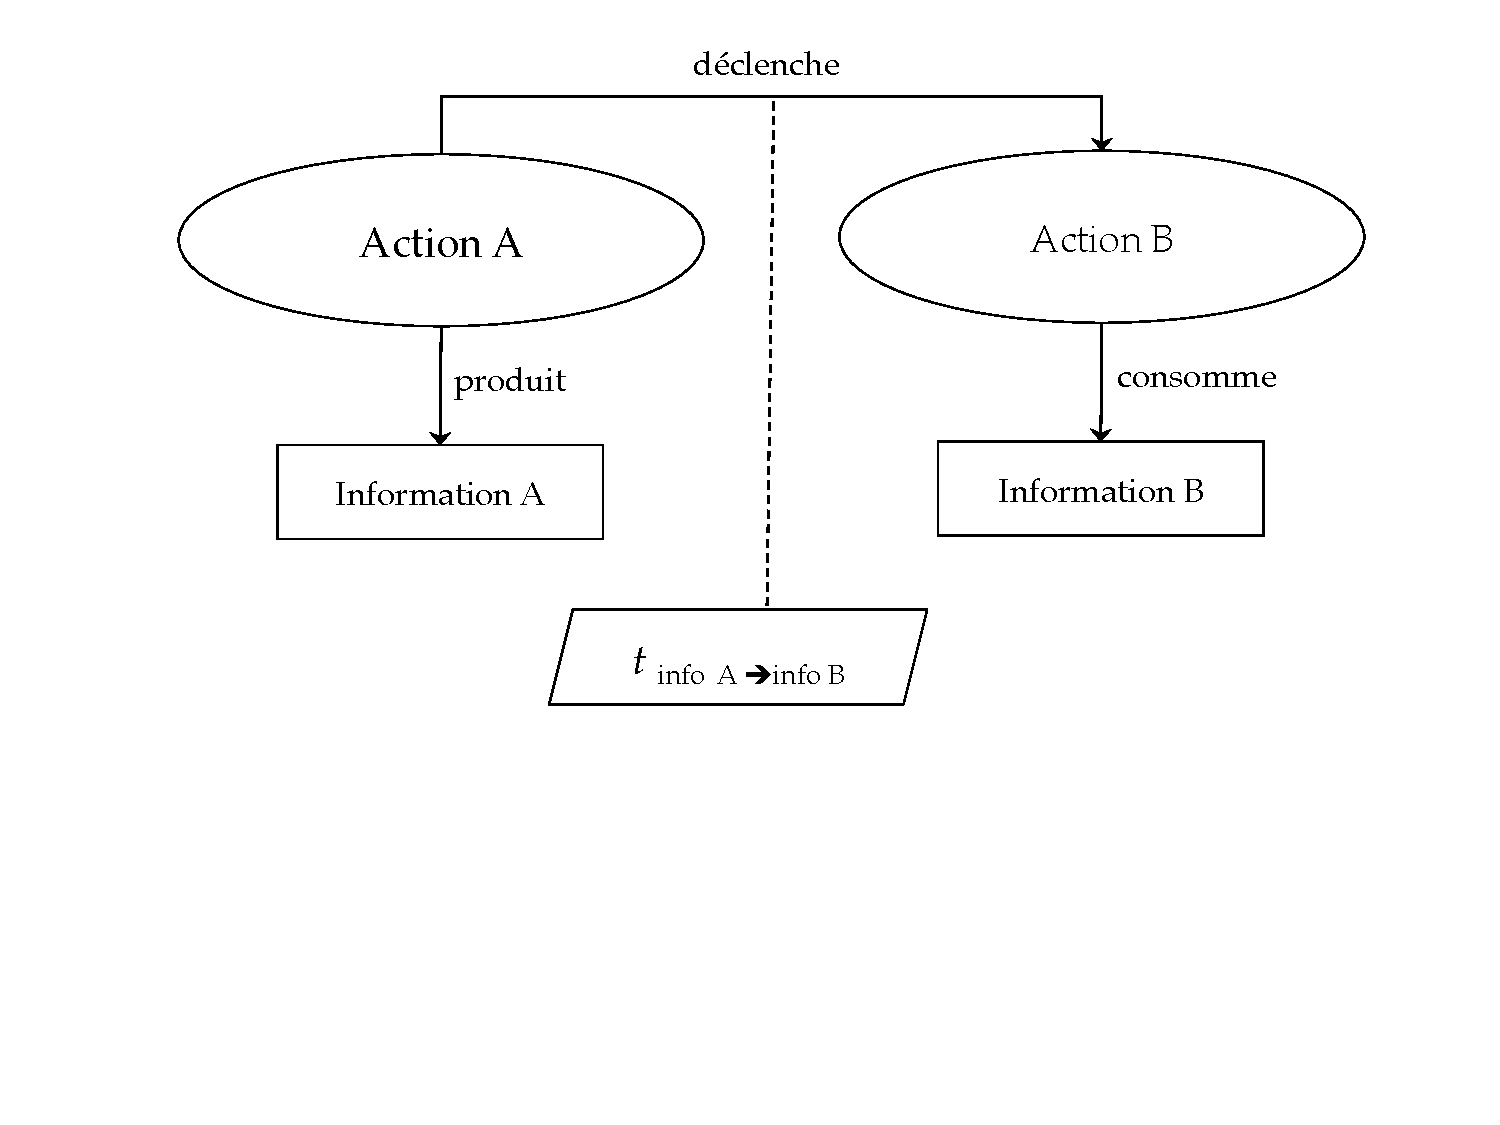
\includegraphics[trim= 0cm 7.5cm 0cm 0cm, width=1\textwidth]{figures/4_demarche/transfo_coherence.pdf}
 \end{center}
 \caption{Identification d'une transformation de modèles\\pour garantir une cohérence intra-vue}
 \label{fig:transfo_coherence}
\end{figure}

La transformation de modèle est un moyen de renforcer l'alignement métier/IT en automatisant le passage d'une vue
à l'autre. Avec les technologies IDM actuelles, il est possible par exemple de transformer une fonction en un code pour
le module applicatif qui l'implémente. Le passage de la vue métier à la vue fonctionnelle demeure quant à lui essentiellement
manuel. L'analyse de la cohérence vise à identifier, dans la vue intégration, ce type de transformation de modèle
et les entités du modèle qu'il concerne.
Les transformation de modèle constituent une solution pour capitaliser le savoir faire métier au niveau des modèles et le rendre
plus indépendant de la plate-forme d'implémentation. Ainsi, il est possible de raisonner au niveau fonctionnel, en modifiant une fonction par exemple, et de réutiliser une transformation de modèle préalablement créée pour re-générer le code du module applicatif cible.

La vue d'intégration offre ainsi la possibilité d'analyser la cohérence de l'architecture d'entreprise
à travers la méta-modélisation, la relation de conformité de l'IDM et les transformations de modèle.
À l'issue de l'analyse de la cohérence de la structure, l'architecture est 

Cette vue donne ainsi accès aux informations de traçabilité qui
permettent de déterminer l'impact d'une modification ou d'une défaillance d'un
module applicatif sur les processus métier. Elle permet aussi de vérifier que
les formats applicatifs permettent d'encoder les types de données fonctionnelles
requis, qui eux-même raffinent les concepts métiers. Cette vue détermine les
éventuelles transformations de modèle nécessaires au déploiement en spécialisant
l'association «~raffine~». Le choix des modèles à transformer dépend fortement
de leur nature (modèles graphiques, textuels, etc.) et mais aussi de leur niveau
d'abstraction. Par exemple, la génération de code demande un modèle en entrée
suffisamment détaillé pour exécuter une transformation pertinente. L'état de
l'art actuel des langages de transformation de modèle privilégie l'usage des
transformations de modèle entre la vue fonctionnelle et et la vue applicative.


ll est indispensable s'assurer de la cohérence
entres les modèles des différentes vues avant d'initier une analyse
d'impact du changement qui soit pertinente pour les parties-prenantes, en particulier
pour l'architecte d'entreprise. L'analyse de l'impact du
changement consiste à dévoiler les effets de bord d'un changement apporté à un
élément de l'architecture.

Dans le contexte du \q{framework ExecuteEA}, l'analyse d'impact exploite les
liens de traçabilité pour identifier les éléments du modèle impacté par une modification 
apportés à une entité du modèle d'architecture. I
L'analyse d'impact évalue par exemple la conséquence de l'indisponibilité d'un module applicatif sur l'architecture
globale~: en mettant à profit les liens de cohérence de la vue intégration, il
est alors possible de déterminer quels sont les processus métier ou
fonctionnels touchés par cette défaillance applicative. De la même manière, il devient
possible d'identifier les modules applicatifs existants pouvant participer à la
réalisation d'un nouveau métier si ces processus fait intervenir des taches
métier déjà implémentées dans le SI.

Nous proposons donc d'analyser les impacts d'exprimer des requêtes sur les modèles
d'architecture et d'étudier le résultat de ces requêtes.Nous proposons
donc de tirer profit des méthodes IDM telle la méta-modélisation et de les
associer à des langages capables d'exprimer et d'exécuter des requêtes sur les modèles d'architecture
tels que OCLinEcore ou QVT.


L'automatisation de l'analyse d'impact est particulièrement cruciale pour les grandes entreprises qui ont à gérer
un patrimoine applicatif important et un nombre de processus métier conséquent.
Il s'agit là d'une analyse statique, le raisonnement concerne uniquement l'aspect structurel. Nous abordons l'analyse
du comportement de la structure dans la suite de ce chapitre.

% Notre contribution consiste à définir la manière dont les langages et techniques
% de l'IDM peuvent être utilisés pour mener une analyse structurelle des modèles
% d'entreprise. Le cadre d'EA que nous proposons permet d'acquérir une vision
% globale et cohérente de l'ensemble des artefacts qui la composent. La taille de
% plus en plus importantes des entreprises actuelle fait que la complexité de
% l'entreprise en tant que système se retrouve dans les modèles d'architecture qui
% le représentent.



% Les langages de modélisation doivent donc permettre de représenter
% convenablement les différents composants de l'entreprise en plus d'offrir la
% possibilité d'analyser la structure des modèles créés dans l'objectif de mieux
% comprendre le système réel, qui est dans ce cas l'entreprise.  Grâce à ce type de langage
% il est possible de~:

% \begin{enumerate}
%     \item modéliser des règles de structure supplémentaires qui précisent d'avantage méta-modèle d'architecture. Une fois
% que le modèle d'architecture est conforme à ce métamodèle, il est possible de
% vérifier qu'il respecte bien toutes les contraintes exprimées au niveau du
% métamodèle~;
%     \item 
%     \end{enumerate}




        \subsubsection{Analyse du comportement : simulation dirigée par les processus
métier}

Comme relaté dans l'état de l'art, l'analyse fait partie des activités les moins
courantes de l'EA quelle qu'en soit l'école de pensée
\cite{chen2008architectures} \cite{barn2013enterprise}. Et même lorsqu'une
architecture d'entreprise est analysée très peu d'approches recourent à la
simulation pour analyser l'aspect comportemental \cite{glazner2011enterprise}
\cite{manzur2015xarchimate}. La simulation est pourtant une technique reconnue
pour évaluer le comportement d'un système et/ou évaluer plusieurs stratégies
concernant son fonctionnement \cite{shannon1975systems}. Notre approche
préconise de simuler les modèles issus de activités de modélisation et
d'intégration afin de les valider ou les critiquer par l'ensemble des acteurs
impliqués dans l'EA.

Pour simuler le comportement d'une entreprise nous nous appuyons sur les modèles
d'architecture d'entreprise préalablement définis par les différentes parties
prenantes. L'EA permet de capturer l'essentiel des composants d'une
entreprise sous forme d'abstraction. Une approche par points de vue guide la
décomposition d'une entreprise en vues pertinentes pour les différents acteurs.
Ces vues apportent une aide supplémentaire à la définition du périmètre des
modèles de simulation. La vue intégration permet en particulier de définir les
liens entres les différentes vues, donc entre les différents modèles de
simulation et de garantir la cohérence et donc la pertinence de la simulation.
Comme les modèles de simulation sont directement dérivés de l'architecture
d'entreprise telle qu'elle est définie par les parties prenantes, elle est
d'autant plus facile à appréhender à comprendre. Ces derniers peuvent aussi
aisément communiquer et échanger autour des résultats de la simulation.

Les modèles d'entreprise doivent offrir un niveau d'abstraction suffisant à la
compréhension, l'analyse et la communication. Les modèles doivent donc permettre
d'abstraire les détails techniques et les nombreuses interconnexions tout en
garantissant la traçabilité et la cohérence de l'ensemble de l'architecture.
Notre approche consiste donc à mettre en lumière les composants et les
relations qui sont critiques pour le comportement de l'ensemble de
l'architecture. En effet, modéliser l'architecture d'une entreprise revient à la
modélisation de systèmes complexes. Herbert Simon \cite{simon1990prediction}
dans ses travaux de modélisation de systèmes complexes affirme que
«~l'approximation judicieuse et non la puissance de calcul d'une machine~» reste
la manière la plus effective d'adresser des systèmes complexes.

La simulation des processus métier est souvent réduite à de la simple animation
visuelle de diagrammes pour vérifier l'orchestration des taches métier. Nous
proposons de piloter la simulation du comportement de l'architecture par le
processus métier. Dans ce cas, le calcul d'une valeur ne se fait pas au niveau
de la tache métier mais du module applicatif qui l'implémente. Le processus
métier est modélisé sous forme de diagrammes d'activité fUML. Dans ce cas les
simulations du comportement de l'architecture d'entreprise est pilotée par les
processus métier qui sont alors responsable d'orchestrer l'ensemble des modèles
comme l'illustre la figure \ref{fig:Simulation_Approche}. 

La simulation est
lancée après l'intégration de l'architecture à travers la création de lien de
cohérences intra-vue et inter-vues. Ces liens sont par la suite utilisés pour
mettre en œuvre la simulation. D'une part, la \textit{Tâche~A} de la figure
\ref{fig:Simulation_Approche} appelle le \textit{Module~A} car le
\textit{Module~A} raffine la \textit{Fonction~A} qui elle-même raffine la
\textit{Tâche~A}. D'autre part, les liens de cohérences intravue garantisse une
compatibilité entre les informations envoyés par la \textit{Tâche~A} et celles
attendues par la \textit{Tâche~B}, de même entre la \textit{Fonction~A} et la
\textit{Fonction~B} et entre le \textit{Module~A} et le \textit{Module~B}.

\begin{figure}[!ht]
    \begin{center}
        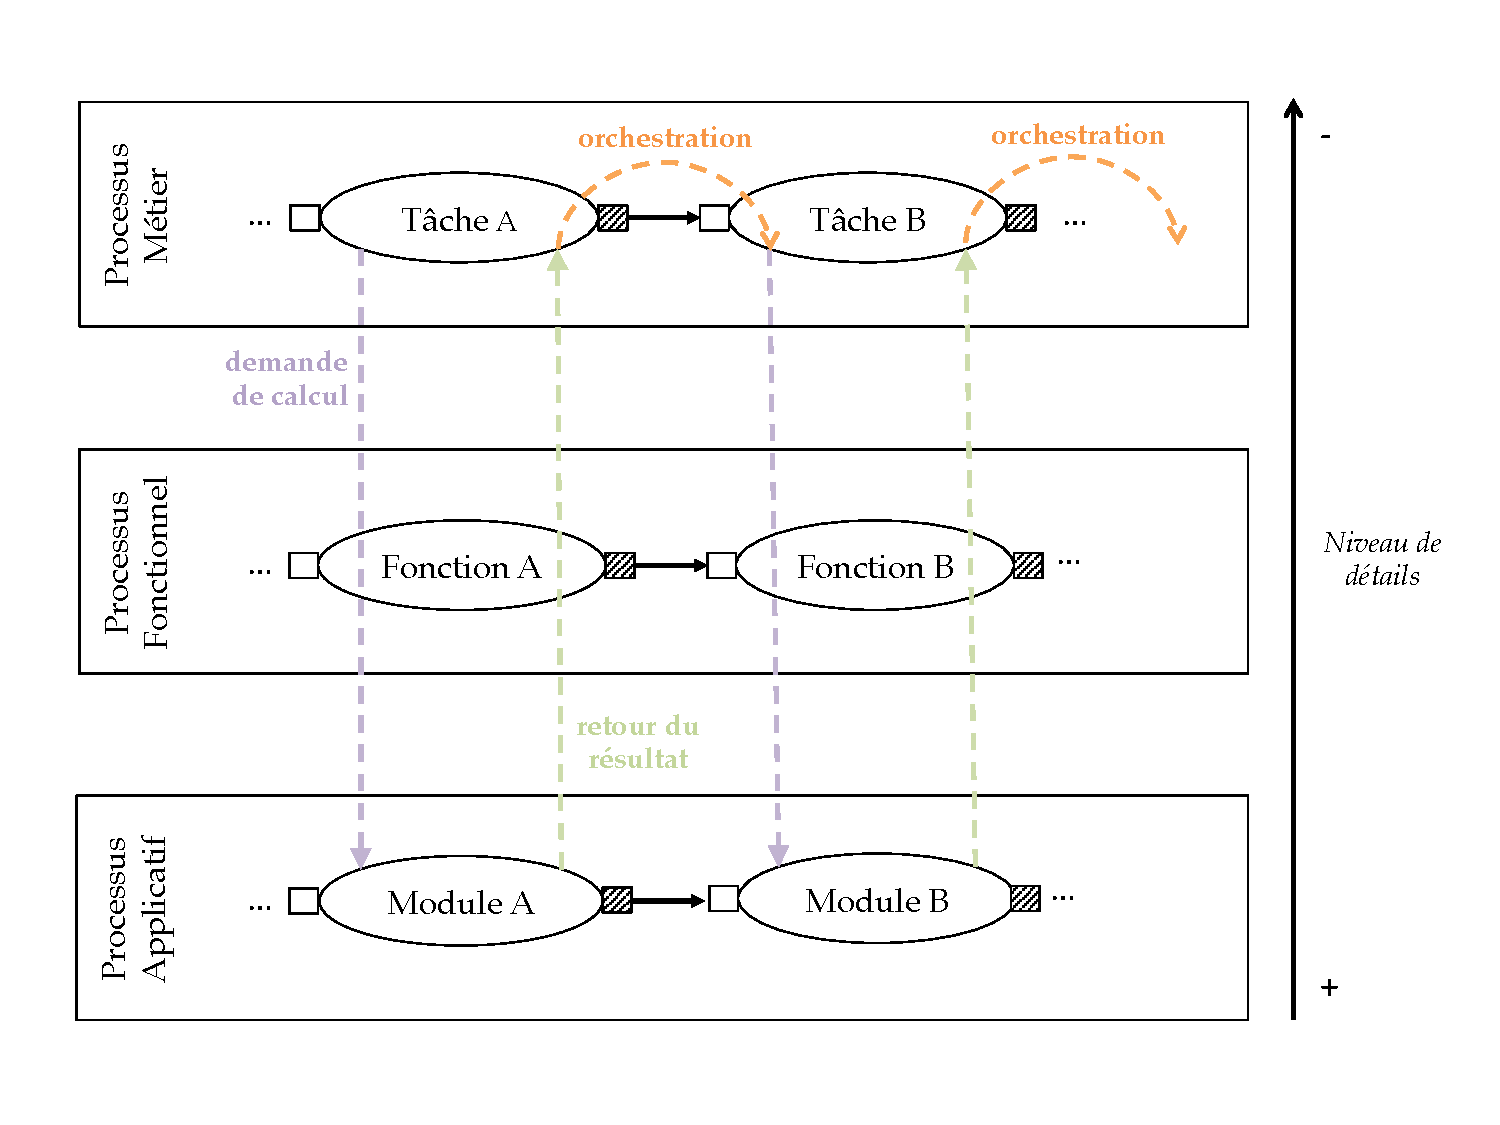
\includegraphics[trim= 0cm 1cm 0cm 0cm, width=1\textwidth]{figures/4_demarche/approche_simulation.pdf}
    \end{center}
    \caption{Simulation de l'architecture dirigée par les processus}
    \label{fig:Simulation_Approche}
\end{figure}

En plus de s'appuyer sur les processus métier pour piloter la simulation de
l'ensemble du comportement de l'architecture d'entreprise, notre approche
consiste à mettre à profit les techniques et les langages de l'IDM pour
faciliter l'automatisation de l'activité d'analyse du comportement. Nous nous
appuyant sur le manifeste de IBM \cite{chesbrough2006research} concernant l'IDM
dans la sélection de techniques et langages qui soient pertinents pour notre
approche. Le manifeste de IBM recommande l'utilisation de langages
(1)~exécutables, (2)~standardisés et (3) compréhensibles par les experts du
domaine. C'est le cas de fUML, BPMN et OCL. La figure \ref{fig:IDM_EA} fait la
correspondance entre les langages et la possibilité de les utiliser selon les
vues.


Ces langages permettent une exécution directe des modèles créés. Contrairement à
d'autres méthodes de simulation de processus métier qui utilisent l'IDM pour
isoler la définition du processus de son exécution. Ces méthodes font ensuite
appel aux transformations de modèle pour automatiser la conversion entre les
modèles de représentation et leur exécution.

\begin{table}[!ht]
    \begin{center}
        \setlength{\mytablewidth}{0.8\textwidth}
\setlength{\mycolwidth}{\dimexpr0.25\mytablewidth-2\tabcolsep\relax}

\begin{tabulary}{\mytablewidth}{m{\mycolwidth}m{\mycolwidth}m{\mycolwidth}m{\mycolwidth}}
\cmidrule[\heavyrulewidth]{2-4}

                        & \centbf{Metier}       & \centbf{Fonctionnel}  & \centbf{Applicatif}   \tabularnewline\midrule
    \centbf{BPMN}       & \center{\checkmark}   &                       &                       \tabularnewline
    \centbf{fUML}       & \center{\checkmark}   & \center{\checkmark}   &                       \tabularnewline
    \centbf{OCL}        &                       & \center{\checkmark}   &                       \tabularnewline
    \centbf{MiniZinc}   &                       &                       & \center{\checkmark}   \tabularnewline

\bottomrule
\end{tabulary}

    \end{center}
    \caption{Langages de l'IDM pour l'EA}
    \label{fig:IDM_EA}
\end{table}

        


















% \begin{figure}[!ht]
%     \begin{center}
%     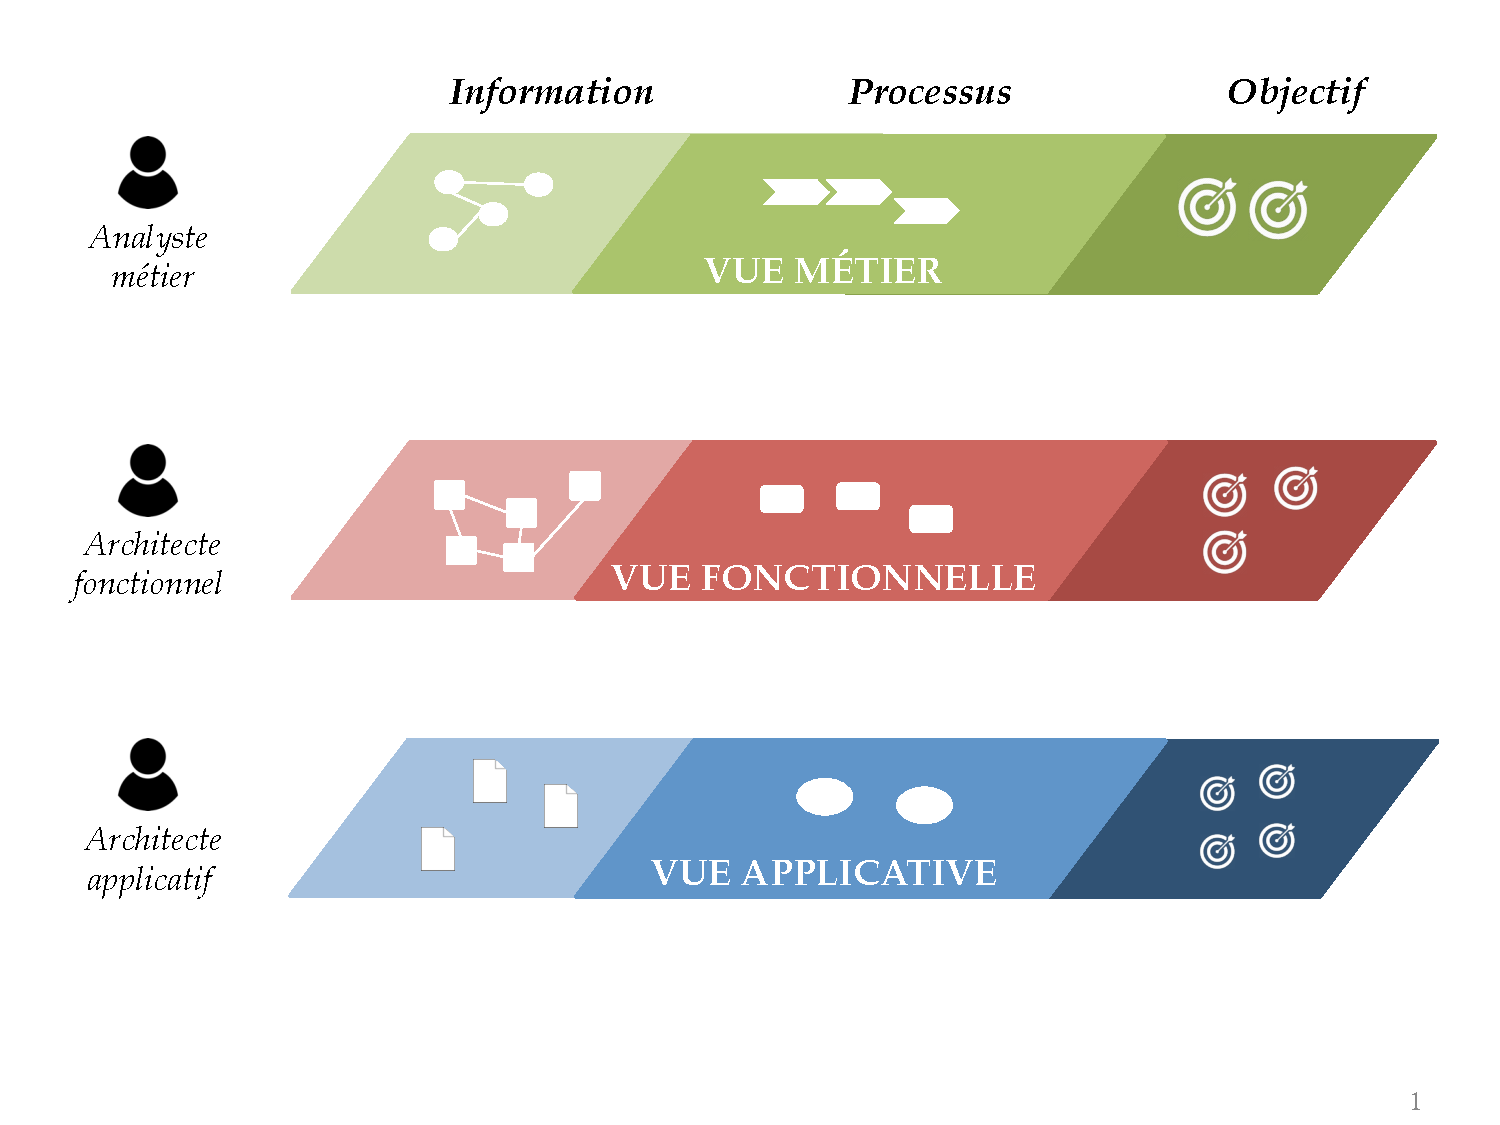
\includegraphics[trim= 0cm 3cm 0cm 0cm, width=1\textwidth]{figures/4_demarche/vue_aspect.pdf}
%     \end{center}
%     \caption{Points de vue et aspects utilisés} \label{fig:vue_aspect}
% \end{figure}

% Nous
% préconisons l'utilisation de formalismes standards pour la modélisation de
% processus métier qui soient exécutables, tels que les diagrammes d'activité \gls{fuml} 
% ou les diagrammes \gls{bpmn} dans une perspective de simulation. Des langages
% spécifiques à un domaine (\gls{dsml}) peuvent également être utilisés~;



% %%(Describes the system’s functional elements, their responsibilities,
%interfaces, and primary interactions. A Functional view is the cornerstone of
%most ADs and is often the first part of the description that stakeholders try
%to %read. It drives the shape of other system structures such as the information
%structure, concurrency structure, deployment structure, and so on. It also has a %significant impact on the system’s quality properties such as its ability to
%change, its ability to be secured, and its runtime performance.) %
%%\subsubsection{Le Model Typing pour la cohérence inter- et intra-vue} %%Le
%\textit{Model Typing} est une technique de l'IDM appliqué au développement
%logiciel permettant de contrôler les types de modèles d'entrée des
%transformations de modèle à leur exécution. Nous proposons d'appliquer les
%principes du \textit{Model Typing} aux modèles d'EA et aux transformations de
%modèle qui leurs sont associées. Par exemple, un processus métier utilise en
%entrée et en sortie des modèles représentant des concepts métier. Un processus
%peut donc être considéré comme une transformation de modèle. %%Ainsi, le
%\textit{Model Typing} peut être utilisé pour l'intégration %horizontale (i.e.
%cohérence et orchestration des processus d'une même vue).

